% =====================================================================
%  A GPU-Batched Parameter-Estimation Toolkit for ABCMB
%  Frequentist profile likelihoods and Sequential Monte Carlo
%  built on the differentiable per-k pipeline.
%
%  Intended audience: the ABCMB authors (Zhou, Giovanetti, Liu).
%  Compile with: pdflatex manual.tex  (run twice for references)
% =====================================================================
\documentclass[11pt]{article}

\usepackage[T1]{fontenc}
\usepackage{lmodern}
\usepackage[margin=1in]{geometry}
\usepackage{amsmath,amssymb,amsfonts}
\usepackage{bm}
\usepackage{booktabs}
\usepackage{longtable}
\usepackage{array}
\usepackage{graphicx}
\usepackage{xcolor}
\usepackage{listings}
\usepackage{enumitem}
\usepackage{microtype}
\usepackage[hidelinks]{hyperref}
\usepackage{caption}
\usepackage{titlesec}

\graphicspath{{../results/}{./}}

% ---- listings style for code / config snippets -----------------------
\definecolor{codebg}{RGB}{245,245,245}
\definecolor{codekw}{RGB}{0,0,160}
\definecolor{codecm}{RGB}{0,128,0}
\lstdefinestyle{py}{
  language=Python, basicstyle=\ttfamily\footnotesize,
  backgroundcolor=\color{codebg}, keywordstyle=\color{codekw},
  commentstyle=\color{codecm}, stringstyle=\color{purple},
  showstringspaces=false, breaklines=true, frame=single,
  framesep=4pt, columns=fullflexible, xleftmargin=4pt, xrightmargin=4pt}
\lstset{style=py}

\newcommand{\code}[1]{\texttt{\small #1}}
\newcommand{\file}[1]{\texttt{\small #1}}
\newcommand{\Neff}{N_{\mathrm{eff}}}
\newcommand{\Cl}{C_\ell}
\newcommand{\Dl}{D_\ell}
\newcommand{\chisq}{\chi^2}
\newcommand{\dchisq}{\Delta\hat\chi^2}
\newcommand{\ginf}{\lVert \bm{g}\rVert_\infty}
\newcommand{\R}{\mathbb{R}}
\newcommand{\Lmax}{\ell_{\max}}
\newcommand{\Tcmb}{T_{\mathrm{CMB}}}
\newcommand{\Bloc}{B_{\mathrm{loc}}}

\titleformat{\paragraph}[runin]{\bfseries}{}{0pt}{}[.]

\title{\textbf{A GPU-Batched Parameter-Estimation Toolkit for \textsc{ABCMB}}\\[4pt]
\large Frequentist Profile Likelihoods and Sequential Monte Carlo\\ on the Differentiable Per-$k$ Pipeline}
\author{Internal technical manual\\ \small for the \textsc{ABCMB} authors (Zhou, Giovanetti \& Liu)}
\date{Compiled \today}

\begin{document}
\maketitle

\begin{abstract}
\noindent
This manual documents a parameter-estimation toolkit built on top of
\textsc{ABCMB}, the differentiable JAX Einstein--Boltzmann solver of
Zhou, Giovanetti \& Liu (arXiv:2602.15104). The toolkit answers a single
operational question: \emph{given a new \textsc{ABCMB}-style cosmology,
return its likelihood optimum and $\pm\,1$--$2\sigma$ confidence
intervals within a few hours of wall clock} --- competitive with, and in
practice faster than, a CLASS+Metropolis--Hastings run of
$\Lambda\mathrm{CDM}+\Neff$ (which takes $\sim22$~h). Two estimators are
provided on \emph{one} likelihood and \emph{one} GPU engine: (i) a
batched, lockstep quasi-Newton \textbf{profile-likelihood} driver that
returns frequentist intervals with per-point automatic-differentiation
stationarity certificates, and (ii) a hand-rolled tempered
\textbf{Sequential Monte Carlo} sampler that returns the Bayesian
posterior and the model evidence. The enabling infrastructure is a
params-axis \emph{batched per-$k$} evaluation of \textsc{ABCMB}
(\code{Model.call\_batched}) that solves many cosmologies at once across
multiple GPUs, and a \emph{staged} forward-mode automatic-differentiation
gradient that threads tangents through the already-compiled batched
stages without ever fusing the cross-device pipeline into a single
intractable program. We give the numerical background, the algorithms,
the custom solvers (the Spectral Projected Gradient foreground profiler,
the fast/slow Gibbs SMC), the parallelism and resource model, and the
production results, including a six-parameter $\Lambda$CDM profile
delivered in $2\,\mathrm{h}\,58\,\mathrm{m}$ on six GPU nodes.
\end{abstract}

\tableofcontents
\clearpage

% =====================================================================
\section{Introduction and scope}
\label{sec:intro}

\subsection{What this toolkit is, and why it exists}

\textsc{ABCMB} computes the lensed CMB temperature/polarization power
spectra $\Cl^{TT},\Cl^{TE},\Cl^{EE}$ and the linear matter power spectrum
$P_m(k)$ for a given cosmology, fully differentiably in JAX, and agrees
with CLASS at the sub-percent level (the published accuracy gate is
$\sim0.2\%$ on TT at $\Lmax=2508$). The solver is the \emph{forward
model}. This manual documents the \emph{inverse} layer built on top of
it: machinery that, given data, returns parameter estimates with
uncertainties.

The design goal, stated by the user verbatim, was:
\begin{quote}
``\emph{I want a tool where I can give it a new cosmology
\textsc{ABCMB}-style and in a few hours I have the optimum $\pm\,1/2\,\sigma$.}''
\end{quote}
The \textbf{competitive bar} is concrete: a CLASS forward model driven by
Metropolis--Hastings (MH) takes roughly $22$~h to map
$\Lambda\mathrm{CDM}+\Neff$ against Planck. A toolkit that needs
node-\emph{days} is not interesting; one that finishes in a few node-hours
\emph{and} carries a convergence certificate MH cannot provide is.

Two estimators are delivered, deliberately on the \emph{same} likelihood
and the \emph{same} forward-model engine so their answers are directly
comparable:
\begin{enumerate}[leftmargin=2em]
\item \textbf{Frequentist profile likelihoods} (Section~\ref{sec:profile}).
For each parameter of interest (POI) we scan a 1-D grid and, at each grid
node, minimise $\chisq$ over all other parameters. The profile curve
$\hat\chisq(\theta_a)$ yields the maximum-likelihood point and
$\dchisq=1,4$ confidence intervals. Every grid node carries an
exact automatic-differentiation (AD) gradient norm as a stationarity
certificate.
\item \textbf{Bayesian Sequential Monte Carlo} (Section~\ref{sec:smc}).
A tempered SMC sampler transports a particle population from the prior to
the posterior, returning marginal posteriors \emph{and} the Bayesian
evidence $Z$ (which a profile scan cannot give). This is the Bayesian
anchor against which the profile is cross-checked, and it supplies the
model-comparison number for extensions.
\end{enumerate}

These two close two specific methodological gaps that a referee of the
\textsc{ABCMB} paper would reasonably raise: a Bayesian posterior +
evidence to anchor the frequentist intervals, and a demonstration that
the differentiable engine enables lockstep batched profiling that is
normally too expensive to run. A third demonstration ---
on-the-batch-axis coverage (Feldman--Cousins/Wilks) mocks, the rigorous
verification that the $\dchisq$ intervals have correct frequentist
coverage --- is described in Section~\ref{sec:coverage}. It is now
\emph{implemented and validated}: the batched coverage validator is built
(\file{scan/wilks.py}), its fitter has been checked on GPU, and the
production $500$-mock runs are underway; an $N\!=\!500$ preview already
shows the empirical test statistic tracking its $\chisq_1$ reference.

\subsection{The single idea that makes it fast}

A conventional CMB likelihood call solves one cosmology at a time, and is
bottlenecked by the slowest Fourier mode $k$ in the perturbation solve.
The \textsc{ABCMB} per-$k$ refactor turns this around: it places many
\emph{cosmologies} on a batch axis and solves one $k$-mode for all of
them at once, looping over $k$. The whole profile grid (or the whole SMC
particle population) is then a single batched forward evaluation, sharded
across the GPUs of a node, and the embarrassingly-parallel batch axis is
where extra grid points and multistarts become nearly free. The
frequentist and Bayesian tools are both thin Python drivers around this
one batched primitive, plus --- for the profile tool --- a \emph{staged}
forward-mode gradient that differentiates the batched pipeline without
ever fusing it.

\subsection{How to read this manual}

Section~\ref{sec:notation} fixes notation; please skim it, because the
two estimators share symbols. Section~\ref{sec:background} is a
self-contained primer on the numerical and statistical methods (profile
vs.\ marginal inference, quasi-Newton and projected-gradient optimisation,
automatic differentiation, SMC, GPU SPMD parallelism); experts may skip
it. Sections~\ref{sec:engine}--\ref{sec:like} document the engine and the
likelihoods. Sections~\ref{sec:profile}--\ref{sec:smc} document the two
tools. Section~\ref{sec:resources} collects the parallelism/resource
model. Section~\ref{sec:rigor} argues the statistical validity (Wilks'
theorem and coverage), the optimiser/sampler convergence guarantees, and
the numerical error budget --- read it if you are weighing the rigor.
Section~\ref{sec:results} gives results (with a consolidated empirical
validation summary, Section~\ref{sec:validation}).
Section~\ref{sec:interface} documents the code interface and gives
copy-paste examples; Section~\ref{sec:usage} is the production cookbook,
Section~\ref{sec:gotchas} the hard-won gotchas, and the appendices
(\ref{app:profenv}, \ref{app:smcenv}, \ref{app:files}) hold the env-var
and file references. Section~\ref{sec:relatedwork} places the work in the
cosmology profile-likelihood literature, and
Section~\ref{sec:improve} lists directions for more precision or speed.

\subsection{Software provenance and constraints}
\label{sec:provenance}

All code lives in the standalone \textsc{ABCMB} checkout
(\file{/pscratch/sd/c/carag/ABCMB-k}); the tool sources are under
\file{scan/}. The engine changes (the batched pipeline, the
\code{expmkappa\_tab} keystone, the sharding helper) live on branch
\code{perk-perf}. Hard constraints honoured throughout, set by the user:
permille-level theory accuracy (no tolerance loosening, no \code{float32},
no mixed precision); production perturbation tolerance
$\mathtt{rtol\_large\_k\_PE}=10^{-5}$; no tight-coupling/regime-switching
hacks in the ODE; $k$-chunk fixed at $100$; massive-neutrino multipole
cutoffs never lowered; SLURM scaling by \emph{nodes}, not walltime, and
never the (2$\times$-charged) premium queue.

\subsection{Related work: frequentist profile likelihoods in cosmology}
\label{sec:relatedwork}

Frequentist profile likelihoods have become a standard cross-check in
cosmology precisely because Bayesian marginal posteriors can be distorted
by \emph{prior-volume effects}: when a model has poorly-constrained
directions (e.g.\ early dark energy as its amplitude
$f_{\mathrm{EDE}}\to0$, or a bounded tensor-to-scalar ratio $r\ge0$),
marginalisation integrates over a large prior volume and can pull the 1-D
posterior away from the best fit, mimicking or hiding a detection. The
profile likelihood, depending only on the maximum of the likelihood at
each POI value, is immune to this. Herold, Ferreira \& Komatsu
\cite{Herold2022} made the point sharply for EDE with Planck+BOSS by
comparing grid sampling and profile likelihoods; the subsequent literature
built dedicated tooling --- Gómez-Valent's fast volume-effect test
\cite{GomezValent2022}, the MCMC-based approximate profiles of Nygaard,
Holm et al.\ and the \textsc{PROSPECT} simulated-annealing optimiser
\cite{Nygaard2023,Holm2024}, and \textsc{Procoli} \cite{Karwal2024} ---
and the method is now applied across extensions (e.g.\ recent
dark-matter--baryon-scattering prior-volume studies \cite{DMb2026}).

The recurring practical obstacles in all of this prior work are exactly the
two that \textsc{ABCMB}'s differentiable, GPU-batched engine removes:
\begin{enumerate}[leftmargin=2em,itemsep=1pt]
\item \textbf{Reliable optimisation.} The inner minimisation over
$\theta_{\setminus a}$ (tens of correlated parameters) is hard, and
CLASS/CAMB provide no gradient, so existing codes lean on gradient-free
global optimisers (simulated annealing) or build an approximate profile
from a pre-existing MCMC --- with no cheap, exact certificate that a
reported minimum is actually a minimum. Here the staged forward-mode AD
gradient (Section~\ref{sec:staged}) gives an exact $\ginf$ at every grid
node, a per-point stationarity certificate, and drives a preconditioned
BFGS that converges in a handful of iterations.
\item \textbf{Affordable density and validation.} A dense grid, multistarts
for global-minimum checks, and coverage mocks (Section~\ref{sec:coverage})
are normally too expensive because each likelihood call is a serial
Boltzmann solve. The per-$k$ batch axis makes them nearly free --- the
whole grid (and, later, hundreds of mock re-fits) is one sharded
\code{call\_batched}.
\end{enumerate}
This work therefore sits in the same methodological lineage as
\cite{Herold2022,Nygaard2023,Holm2024,Karwal2024} but replaces the
gradient-free, one-cosmology-at-a-time backend with a differentiable,
batched one: it trades the simulated-annealing heuristic for an
AD-certified quasi-Newton descent, and turns the coverage validation those
works flag as desirable-but-expensive into a routine batch job.

% =====================================================================
\section{Notation and conventions}
\label{sec:notation}

We use the following symbols consistently throughout. The single most
common source of confusion is the word ``nuisance,'' which is overloaded
in CMB analysis; we reserve it for the \emph{instrumental/foreground}
parameters of the likelihood and use ``co-profiled parameters'' for the
cosmological parameters minimised away in a profile.

\begin{longtable}{p{0.16\textwidth}p{0.78\textwidth}}
\toprule
Symbol & Meaning \\
\midrule
\endhead
$\theta$ & Cosmological parameter vector, $\theta\in\R^{D}$, components in
a fixed \emph{order} (Section~\ref{sec:config}). \\
$D$ & Number of cosmological parameters being varied
($D=6$ for base $\Lambda$CDM; $D=7$ for $\Lambda\mathrm{CDM}+\Neff$). When
instrumental nuisances are also \emph{sampled} (the full-\code{plik} SMC),
the total sampled dimension is written explicitly as $D+21$
(``$27$-dimensional''), never as $D$. \\
$\theta_a$ & A \emph{parameter of interest} (POI); $a$ is its index in
the order, used consistently as the POI index. \\
$\theta_{\setminus a}$ & The remaining $D-1$ cosmological parameters,
\emph{co-profiled} (minimised over) at fixed $\theta_a$. \\
$P$ & Number of co-profiled cosmological parameters in a profile row,
$P=D-1$. (Distinct from the matter power $P_m(k)$ and the per-multipole
probability $P_\ell$, which always carry their argument.) \\
$\bar\theta$ & Fiducial centre vector (config \code{cen}; the array
\code{CENTER}). \\
$\sigma$ & Per-parameter prior-scale widths (config \code{sig}; the array
\code{SIGMA}). $\sigma$ non-dimensionalises the optimiser; it also
\emph{defaults} as the grid half-extent unit, but the grid half-span is
replaced by the MLE Fisher errors when the MLE pre-pass is enabled
(Section~\ref{sec:mle}). \\
$\bm{x}$ & Scaled (dimensionless) optimisation coordinates,
$x_k=(\theta_{i_k}-\bar\theta_{i_k})/\sigma_{i_k}$ for the $k$-th
co-profiled parameter; $\bm{x}\in\R^{P}$, box-constrained to
$[-x_{\mathrm{box}},x_{\mathrm{box}}]$ with $x_{\mathrm{box}}=5$. \\
$\nu$ & Instrumental/foreground \emph{nuisance} parameters of the
likelihood; $\nu\in\R^{21}$ for full Planck \code{plik}, or the single
calibration $A_{\mathrm{planck}}$ for \code{plik\_lite}. \\
$\mathcal{D}$ & Data (the binned bandpowers / low-$\ell$ likelihood
inputs); $\bm{\mathcal{D}}$ is the \code{plik\_lite} data bandpower
vector. \\
$\Cl^{XY}$ & Theory angular power spectra, $XY\in\{TT,TE,EE\}$,
dimensionless as produced by \textsc{ABCMB}. \\
$\Dl^{XY}$ & $\Dl=\ell(\ell+1)\,\Cl\,\Tcmb^2/2\pi$ in $\mu\mathrm{K}^2$,
with $\Tcmb=2.7255\times10^{6}\,\mu\mathrm{K}$. \\
$\chisq(\theta,\nu)$ & The total chi-squared $=-2\ln L$, summed over
high-$\ell$ + low-$\ell$ TT/EE contributions. \\
$\chisq_{\mathrm{prof}}(\theta)$ & $\chisq$ with the instrumental
nuisances $\nu$ profiled out: $\min_\nu\chisq(\theta,\nu)$
(Section~\ref{sec:envelope}). \\
$\hat\chisq(\theta_a)$ & The \emph{profile likelihood}:
$\min_{\theta_{\setminus a}}\chisq_{\mathrm{prof}}(\theta)$, the deliverable
curve for POI $a$. \\
$\dchisq$ & $\hat\chisq(\theta_a)-\min_{\theta_a}\hat\chisq$, the profile
offset from its minimum; abbreviated $\Delta\chisq$ in figures/tables. \\
$\bm{g}$ & Gradient of the (scaled) objective,
$\bm{g}=\nabla_{\bm x}\,\chisq_{\mathrm{prof}}$; $\ginf$ is its
$\ell_\infty$ norm, the stationarity certificate. \\
$\bm{H}^{-1}$ & The BFGS inverse-Hessian estimate (the array \code{Hinv}). \\
$\bm{d}$ & Optimiser search direction, $\bm d=-\bm H^{-1}\bm g$. \\
$\sigma_1$ & The $\dchisq=1$ profile interval half-width for a POI;
the quantity the early-stop monitors. \\
$\mathrm{GTOL}$ & Gradient-norm convergence threshold,
$\ginf<\mathrm{GTOL}$ (default $3\times10^{-2}$). \\
$\beta$ & SMC inverse temperature, $\beta:0\!\to\!1$. \\
$N$ & Number of SMC particles (fixed for a run; default $512$). \\
$M$ & SMC random-walk moves per stage ($M=3$ for \code{plik\_lite};
$M_{\mathrm{slow}}=2$, $M_{\mathrm{fast}}=20$ for the full-\code{plik}
fast/slow split). \\
$w_i,\ \bm{W}$ & $w_i$ the normalised SMC weight of particle $i$
($\mathrm{ESS}=1/\sum_i w_i^2$); $\bm W$ the cumulative (un-normalised)
importance weights, so $\log\bm W$ is the running log-weight array. \\
$Z$ & Bayesian evidence; $\log Z$ is accumulated from the SMC normalising
constants. \\
$B$ & Batch size: number of cosmologies in one
\code{call\_batched}. For the profile tool a batch \emph{row} is one
$(\theta_a,\text{grid value})$ pair, so $B$ is also the number of profile
rows. \\
$\Bloc$ & Per-device batch size, $\Bloc=B/n_{\mathrm{dev}}$ after
sharding across $n_{\mathrm{dev}}$ GPUs. \\
$\Lmax$ & Maximum multipole of the theory solve (production $2508$). \\
\bottomrule
\end{longtable}

\paragraph{Base-$\Lambda$CDM parameter order}
The canonical order for base $\Lambda$CDM is
\[
\theta=\bigl(h,\ \omega_b,\ \omega_c,\ n_s,\ \mathcal{A}_s,\ \tau\bigr),
\]
where $\omega_b\equiv\Omega_b h^2$, $\omega_c\equiv\Omega_c h^2$
(``\code{omega\_cdm}''), $\mathcal{A}_s\equiv\ln(10^{10}A_s)$
(``\code{ln10As}''), $\tau\equiv\tau_{\mathrm{reion}}$, and $h$ is the
reduced Hubble constant ($H_0\equiv100\,h\,\mathrm{km\,s^{-1}Mpc^{-1}}$;
we use $h$ everywhere). Internally \textsc{ABCMB} receives
$A_s=\exp(\mathcal{A}_s)/10^{10}$; every other parameter passes through by
name. Extensions append parameters (e.g.\ $\Neff$ with fiducial $3.044$).

% =====================================================================
\section{Background: numerical and statistical foundations}
\label{sec:background}

This section is a self-contained primer. Readers fluent in quasi-Newton
and projected-gradient optimisation, automatic differentiation,
profile-likelihood theory, and sequential Monte Carlo may skip to
Section~\ref{sec:engine}.

\subsection{Profile vs.\ marginal inference}
\label{sec:profvsmarg}

Given a likelihood $L(\theta,\nu)=\exp[-\tfrac12\chisq(\theta,\nu)]$, two
philosophies reduce the high-dimensional surface to a statement about one
parameter $\theta_a$.

\emph{Frequentist profiling} maximises out the other parameters:
\begin{equation}
\hat\chisq(\theta_a)=\min_{\theta_{\setminus a},\,\nu}
\chisq(\theta_a,\theta_{\setminus a},\nu).
\label{eq:profdef}
\end{equation}
By Wilks' theorem, for a well-behaved model the profile offset
$\dchisq(\theta_a)\equiv\hat\chisq(\theta_a)-\min_{\theta_a}\hat\chisq$
[Eq.~\eqref{eq:profdef}] is asymptotically $\chisq$-distributed with one
degree of freedom, so the $1\sigma$ ($2\sigma$) confidence interval is the
set where $\dchisq\le1$ ($\le4$). Profiling makes no prior assumption on
the co-profiled parameters and is reparametrisation-covariant in the POI.

\emph{Bayesian marginalisation} integrates them out:
$p(\theta_a\mid\mathcal D)\propto\int
L(\theta,\nu)\,\pi(\theta,\nu)\,\mathrm d\theta_{\setminus a}\,\mathrm d\nu$,
with prior $\pi$. The marginal depends on the prior and on volume effects;
the profile does not. For Gaussian, unimodal posteriors the two agree;
where they disagree (e.g.\ a parameter bounded against a physical edge,
or a strong degeneracy such as $\Neff$--$\omega_c$--$h$) the
\emph{difference itself} is a result. Delivering both on one likelihood is
therefore scientifically, not just methodologically, motivated.

\subsection{The envelope theorem: profiling nuisances cheaply and exactly}
\label{sec:envelope}

The CMB likelihood carries instrumental/foreground nuisances $\nu$
(Section~\ref{sec:like}). Re-solving the Boltzmann hierarchy every time a
foreground amplitude moves would be wasteful: $\nu$ does not change the
theory $\Cl$. We therefore profile $\nu$ \emph{inside} the likelihood at
fixed theory,
\begin{equation}
\chisq_{\mathrm{prof}}(\theta)=\chisq\bigl(\theta,\nu^\star(\theta)\bigr),
\qquad
\nu^\star(\theta)=\arg\min_\nu\chisq(\theta,\nu).
\end{equation}
The \textbf{envelope theorem} states that, at the inner optimum
$\nu^\star$ where $\partial\chisq/\partial\nu=0$,
\begin{equation}
\frac{\mathrm d\,\chisq_{\mathrm{prof}}}{\mathrm d\theta}
=\frac{\partial\chisq}{\partial\theta}\Bigl(\theta,\nu^\star(\theta)\Bigr)
+\underbrace{\frac{\partial\chisq}{\partial\nu}\frac{\mathrm
d\nu^\star}{\mathrm d\theta}}_{=\,0},
\end{equation}
so the gradient of the profiled objective with respect to cosmology is
just the partial derivative at the frozen $\nu^\star$. In code this is
realised by \code{stop\_gradient($\nu^\star$)}: we differentiate
$\chisq$ in $\theta$ holding $\nu^\star$ fixed, never back-propagating
through the inner optimiser. This makes the cosmology gradient exact
\emph{and} cheap, and is the mechanism that lets a 21-parameter
foreground profile sit inside an AD-differentiable cosmology likelihood.

\subsection{Quasi-Newton optimisation: BFGS, line search, preconditioning}
\label{sec:bfgs}

At each profile grid node we minimise a smooth $\chisq(\bm x)$ over the
$P$ scaled co-profiled coordinates. Newton's method needs the Hessian;
for the CMB likelihood at $\Lmax=2508$ a full AD Hessian is prohibitive
(forward-over-forward costs $\sim35$~GB per cosmology). The
\textbf{BFGS} quasi-Newton method instead builds an inverse-Hessian
estimate $\bm H^{-1}$ from successive gradient pairs. With step
$\bm s=\bm x_{k+1}-\bm x_k$ and gradient change $\bm y=\bm
g_{k+1}-\bm g_k$, and $\rho=1/(\bm s^\top\bm y)$,
\begin{equation}
\bm H^{-1}_{k+1}=
(\bm I-\rho\,\bm s\bm y^\top)\,\bm H^{-1}_k\,(\bm I-\rho\,\bm y\bm
s^\top)+\rho\,\bm s\bm s^\top,
\label{eq:bfgs}
\end{equation}
applied only when the curvature condition holds. We use the
\emph{relative} safeguard $\bm s^\top\bm y>10^{-8}\,\lVert\bm
s\rVert\,\lVert\bm y\rVert$ rather than an absolute floor, because near
convergence $\bm s,\bm y\to0$ and an absolute test corrupts $\bm H^{-1}$
with noise. The search direction is $\bm d=-\bm H^{-1}\bm g$, reset to
steepest descent $\bm d=-\bm g$ (and $\bm H^{-1}=\bm I$) if it fails to be
a descent direction ($\bm g^\top\bm d\ge0$).

\paragraph{Line search}
We accept a step length $\alpha$ by the \textbf{Armijo} sufficient-decrease
condition,
\begin{equation}
\chisq(\bm x+\alpha\bm d)\le\chisq(\bm x)+c_1\,\alpha\,\bm g^\top\bm d,
\qquad c_1=10^{-4},
\label{eq:armijo}
\end{equation}
backtracking $\alpha\to\alpha/2$ up to $12$ times. A subtle but important
rule (the ``consistency rule,'' Section~\ref{sec:consistency}) is that
\emph{every} $\chisq$ value entering Eq.~\eqref{eq:armijo} --- the
reference, the trial, and the recorded profile --- comes from one
evaluation path; gradients come from a separate path. Mixing value
sources makes the line search inconsistent and stalls BFGS.

\paragraph{Preconditioning}
Steepest descent on the ill-conditioned CMB likelihood (the co-profiled
Hessian has condition numbers $\sim32$--$159$ across POIs) is hopeless;
the first BFGS step from an identity $\bm H^{-1}$ is a steepest-descent
step. We therefore initialise $\bm H^{-1}_0$ from the inverse of the
co-profiled submatrix of the $\chisq$ Hessian evaluated at the warm-start
point (the global best fit / joint MLE; Section~\ref{sec:mle}) --- an
inverse-Fisher preconditioner. This makes the first iteration near-Newton
and is what lets BFGS descend the valley rather than oscillate across it.

\subsection{Bound-constrained projected gradient: BB steps and nonmonotone line search}
\label{sec:spgbg}

The \emph{inner} foreground profiler (Section~\ref{sec:spg}) is a
different optimiser, because its objective (clipy) supplies a reliable
first derivative but \emph{not} a usable Hessian, and several nuisances
sit against hard bounds. The right tool is a \textbf{Spectral Projected
Gradient} (SPG) method, which needs only gradients and respects a box.
Its three ingredients:
\begin{itemize}[leftmargin=1.5em,itemsep=2pt]
\item \emph{Projected step.} For a box $[\bm z_{\mathrm{lo}},\bm
z_{\mathrm{hi}}]$, the search direction is
$\bm d=\Pi_{[\bm z_{\mathrm{lo}},\bm z_{\mathrm{hi}}]}(\bm z-\alpha\bm
g)-\bm z$, where $\Pi$ is the (cheap) projection onto the box. A parameter
that wants to leave the box is pinned exactly at the bound --- essential
when, e.g., a kSZ amplitude rails at zero.
\item \emph{Barzilai--Borwein (BB) spectral step.} The step length is
$\alpha=\bm s^\top\bm s/\bm s^\top\bm y$ (with $\bm s,\bm y$ the latest
coordinate/gradient changes), a scalar approximation to the inverse
Hessian curvature built from two consecutive gradients --- so no Hessian
is ever formed.
\item \emph{Nonmonotone line search.} Rather than requiring decrease
against the current value, the Grippo--Lampariello--Lucidi (GLL) criterion
accepts a step that decreases against the \emph{maximum} of the last few
objective values. This lets the BB step take occasional uphill moves that
accelerate convergence on curved valleys --- the practical key to SPG's
speed over a monotone backtracking search.
\end{itemize}
SPG converges like a bound-constrained L-BFGS-B but uses only first
derivatives, which is exactly the regime the clipy foreground profile
lives in.

\subsection{Automatic differentiation: forward vs.\ reverse mode}
\label{sec:ad}

Automatic differentiation evaluates exact derivatives of a program by
the chain rule, without finite-difference truncation error.
\emph{Forward mode} (the Jacobian--vector product, jvp) propagates a
tangent $\dot{\bm x}$ forward through the program, returning
$\bm J\dot{\bm x}$ in one pass; computing the full gradient of a
scalar in $P$ inputs costs $P$ forward passes. \emph{Reverse mode} (the
vector--Jacobian product, vjp) propagates a cotangent backward, returning
the full gradient of a scalar in one pass but requiring the entire
forward trace to be stored.

For this toolkit forward mode is the right choice, for two reasons.
First, the cost: $P$ forward directions cost about the same as a $P$-point
finite-difference (FD) stencil, and we typically need only $P=D-1\le6$
directions. Second, and decisively, reverse-mode through the
\textsc{ABCMB} pipeline would require tracing the entire cross-device
(GPU$\to$CPU$\to$GPU) solve as one program, which is exactly the
intractable monolith we avoid (Section~\ref{sec:staged}). Forward mode
lets us differentiate \emph{stage by stage}.

\paragraph{Why exact gradients matter}
A central FD gradient is only as good as its step size. At the steep
curvature near a profile minimum, FD was measured to be $1$--$7\%$ wrong,
and worse, it can simultaneously \emph{fake} stalls (noise spikes that
look like a large residual gradient) and \emph{fake} convergence (noise
cancellation that makes an unconverged point look stationary). Indeed the
shipped $\Lambda$CDM config was switched to exact-AD iterations precisely
because FD calibration could not clear its noise floor at full $\ell$
(Section~\ref{sec:advsfd}). The exact AD gradient has no truncation floor,
so $\ginf$ can be driven to a genuine stationarity statement --- it is the
convergence \emph{certificate} regardless of which gradient drove the
descent.

\subsection{Sequential Monte Carlo: tempering, resampling, evidence}
\label{sec:smcbg}

SMC transports a population of $N$ weighted particles through a sequence
of distributions bridging an easy reference (the prior) to the target
(the posterior). We use a \textbf{tempered} (annealed) path,
\begin{equation}
\pi_\beta(\theta,\nu)\;\propto\;\pi_{\mathrm{prior}}(\theta,\nu)\;
L(\theta,\nu)^{\beta},\qquad \beta:0\to1,
\end{equation}
so $\pi_0$ is the prior and $\pi_1$ the posterior. (For the
full-\code{plik} sampler the state $(\theta,\nu)$ includes the $21$
foreground nuisances, which are thereby marginalised by sampling; for the
\code{plik\_lite} sampler $\nu=A_{\mathrm{planck}}$ is profiled out and
the state is $\theta$ alone.) At each stage the inverse temperature
advances $\beta\to\beta+\Delta\beta$; the incremental importance weight of
particle $i$ is
\begin{equation}
\log w^{\mathrm{incr}}_i=-\tfrac12\,\Delta\beta\,\chisq_i .
\end{equation}
$\Delta\beta$ is chosen \emph{adaptively} by bisection so that the
effective sample size after reweighting equals a target fraction of $N$
(here $\tfrac12N$): too large a step collapses the weights, too small a
step wastes compute. When the ESS of the cumulative weights falls below
the target we \textbf{resample} (systematic resampling) to refresh the
population, then \textbf{move} each particle with a few random-walk
Metropolis steps that leave $\pi_\beta$ invariant, using a proposal
covariance scaled by the optimal factor $2.38^2/d$ (for a block of
dimension $d$) times the weighted particle covariance. The
\textbf{evidence} comes for free: with $\bm W$ the cumulative
(un-normalised) weights (so $\log\bm W$ is the running log-weight array),
each stage multiplies the population by its mean incremental weight, and
\begin{equation}
\log Z=\sum_{\mathrm{stages}}\Bigl[\,
\mathrm{logsumexp}(\log\bm W+\log\bm w^{\mathrm{incr}})
-\mathrm{logsumexp}(\log\bm W)\Bigr],
\label{eq:logz}
\end{equation}
where the bracket reduces to $\log\overline{w^{\mathrm{incr}}}$ right after
a resample (uniform $\bm W$).

SMC has three properties that suit the batched engine perfectly: it is
\emph{population-based} (every particle is evaluated at once, i.e.\ one
\code{call\_batched}), it has a \emph{fixed} population size (one compiled
batch shape for the whole run), and it yields the evidence at no extra
cost. It is also robust to multimodality and to the GPU$\to$CPU$\to$GPU
non-jittability of \textsc{ABCMB} (Section~\ref{sec:engine}), because the
driver lives in eager Python and only the per-particle likelihood is
batched.

\subsection{GPU parallelism: SPMD, sharding, and the batch axis}
\label{sec:spmd}

A single A100 GPU is a throughput device: it is most efficient when given
a large, regular, data-parallel workload. The per-$k$ refactor exposes
exactly that --- the cosmology batch axis $B$ --- so that one GPU solves
many cosmologies with the same instruction stream (SPMD). To use the four
GPUs of a Perlmutter node we \emph{shard} the batch axis: JAX's GSPMD
partitioner splits the $B$ axis across devices, each device building and
solving $\Bloc=B/n_{\mathrm{dev}}$ cosmologies. Because the pipeline is
embarrassingly parallel over $B$ (no cross-cosmology coupling), there are
\emph{no} collective communications --- the partitioning is a pure data
split. Beyond a node, we scale the tools whose work axis genuinely
decouples by slicing that axis across nodes (one SLURM job, one worker per
node, no MPI gather): the \emph{profile} tool slices its POI list
(Section~\ref{sec:poislice}), and the coverage validator slices
the mock list (Section~\ref{sec:coverage}). The \emph{SMC} sampler does
\emph{not} node-slice --- its tempering, resampling, and weighted
covariance couple the whole particle population --- so it scales only
within a node, sharded across the four GPUs. This (shard within a node,
and slice across nodes where the axis allows) is the parallelism backbone.

% =====================================================================
\section{The engine: batched per-$k$ evaluation and the staged gradient}
\label{sec:engine}

This section documents the forward-model infrastructure the tools sit on:
the batched pipeline \code{Model.call\_batched}, the keystone change that
made it possible, the multi-GPU sharding, and the staged AD gradient.
These live in \file{abcmb/main.py}, \file{abcmb/perturbations.py},
\file{abcmb/spectrum.py}, \file{abcmb/background.py}, and
\file{scan/batched\_grad.py}.

\subsection{The single-cosmology pipeline and its device split}
\label{sec:pipeline}

\textsc{ABCMB} is orchestrated by \code{abcmb.main.Model}, an
\code{eqx.Module}. A call \code{Model(**specs)(params)} runs four
stages with a \emph{deliberate} CPU/GPU split:
\begin{enumerate}[leftmargin=2em,itemsep=2pt]
\item \code{add\_derived\_parameters} (CPU, Python): fills defaults,
resolves the $\Neff$/$N_{\nu,\mathrm{massless}}$/$Y_{\mathrm{He}}$
triangle, and selects the BBN branch (user-supplied $Y_{\mathrm{He}}$,
PArthENoPE table, or bundled LINX).
\item \code{get\_BG\_pre\_recomb} (GPU, \code{eqx.filter\_jit}): tabulates
conformal time and packs the recombination inputs.
\item HyRex recombination (CPU, \code{filter\_jit(\dots, backend='cpu')}):
solves $x_e$, $T_m$ sequentially; outputs are moved back to GPU.
\item \code{\_run\_post\_recomb} (GPU): builds the full background
(reionisation, optical depth, decoupling), runs the perturbation
hierarchy through \code{diffrax}, integrates the line-of-sight transfer,
returns $\Cl$ and $P_m(k)$.
\end{enumerate}
HyRex (and LINX) run on CPU even when GPUs are present: their solvers are
sequential and cheap, and keeping them on CPU avoids serialising the GPU.
This GPU$\to$CPU$\to$GPU structure is the central fact that shapes
everything downstream (Section~\ref{sec:nonjit}).

\subsection{\texttt{Model.call\_batched}: the params-axis batched pipeline}
\label{sec:callbatched}

\code{Model.call\_batched(params\_list, shard=None, k\_chunk\_size=100)}
evaluates a \emph{list} of $B$ cosmologies in lockstep and returns a
\code{BatchedOutput} (the stacked $\Cl^{TT},\Cl^{TE},\Cl^{EE}$, $P_m(k)$,
the $\ell$ and $k$ grids, and the per-cosmology derived params; the
background and perturbation tables are \emph{not} stored, to save memory).
The stages mirror the single-cosmology pipeline but each is vmapped:

\begin{enumerate}[leftmargin=2em,itemsep=2pt]
\item Derive params eagerly: \code{full\_ps = [add\_derived\_parameters(p)
for p in params\_list]}. This stays a Python loop --- it contains
\code{sys.exit} input checks, per-species Python loops, BBN
\code{if/elif} branching, and a CPU LINX call, all hostile to \code{vmap}
--- but it costs only $\sim$ms per cosmology. Unknown keys are wrapped as
\code{jnp.array} so a new physics parameter does not trigger a
recompilation.
\item \code{\_build\_bgs\_batched}: builds the stacked \code{Background}.
Internally it runs three vmapped sub-stages with two device transfers:
\code{\_pre\_recomb\_batched} (GPU, \code{vmap} of
\code{BackgroundPreRecomb}); the HyRex \code{RecModel} (CPU, \code{vmap},
via a \emph{cached} \code{filter\_jit} wrapper \code{\_recmodel\_cpu} ---
the cache is essential, as creating a fresh wrapper per call leaked host
memory until an LLVM allocation failure); and \code{\_get\_BG\_batched}
(GPU, \code{vmap} of \code{get\_BG}). Integer/bool leaves are cast to
\code{float64} \emph{after} stacking, before the GPU stages run.
\item \code{PE.full\_evolution\_batched((BG\_batch, params\_batch),
k\_chunk\_size=100)}: the batched perturbation solve. The $k$-axis is cut
into chunks of $100$ modes; each chunk is a double \code{vmap}
($\code{vmap}_{k}\times\code{vmap}_{B}$) around \code{evolution\_one\_k}
inside a \code{filter\_jit}'d \code{\_evolve\_chunk}, and the chunks are
concatenated along the (unsharded) $k$ axis. The chunk loop is plain
Python, not \code{lax.scan}, because scanning around \code{diffrax}
triggered a $\sim$13-minute compile pathology.
\item \code{SS.get\_Cl\_batched} and \code{SS.Pk\_lin\_batched}: a single
\code{filter\_jit}'d \code{jax.vmap} over $B$ of the line-of-sight
integral and the matter $P_m(k)$, replacing what used to be a Python loop.
\end{enumerate}

The measured win was not solver tuning: it was eliminating two
flat eager-dispatch costs (the spectrum Python loop, and running
\code{get\_BG} eagerly), which collapsed $3B$ JIT dispatches $+\,2B$
device transfers into $3$ JITs $+\,3$ transfers.

\subsection{The keystone: \texttt{expmkappa\_tab}}
\label{sec:keystone}

The change that \emph{enabled} stacking \code{Background} across
cosmologies is small but load-bearing. Previously the background stored
\code{kappa\_func}, a \code{diffrax.Solution} for the optical depth ---
an object with non-array internals that cannot be \code{jnp.stack}'d, so
the batched spectrum had to fall back to a Python loop. It is replaced by
\code{expmkappa\_tab}: $\exp(-\kappa)$ tabulated on a fixed shared axis
\code{lna\_tau\_tab} ($10^4$ points), read back via
\code{interpax.interp1d(method="cubic")}:
\begin{equation}
\exp(-\kappa)(\ln a)\;\approx\;
\mathrm{interp1d}\bigl(\ln a;\ \text{\code{lna\_tau\_tab}},\ \text{\code{expmkappa\_tab}}\bigr).
\end{equation}
Cubic (not linear) interpolation is required because $\Cl^{TE}$ depends on
the gradient of the visibility function $g_v(\ln a)=\exp(-\kappa)/\tau_c$
(with $\tau_c$ the Thomson collision time, $1/\tau_c=\dot\kappa$), which
must stay $C^1$; a piecewise-linear table gives a discontinuous gradient
that corrupts $\Cl^{TE}$ at the $\sim10^{-1}$ level. With this change
\code{Background} becomes a pure-array PyTree, so a single \code{BG\_batch}
stacks across cosmologies and feeds both the perturbation solve and the
spectrum vmap. This is the single edit that unlocks the entire batched
pipeline and the staged gradient.

\subsection{Multi-GPU sharding: \texttt{\_make\_shardfn}}
\label{sec:sharding}

A single helper, \code{Model.\_make\_shardfn(shard)}, defines the entire
sharding policy and is shared verbatim by the primal and the gradient so
both partition $B$ identically. It builds one device mesh over the
visible GPUs and returns a function that places array leaves (schematic):
\begin{lstlisting}
mesh = Mesh(np.asarray(jax.devices('gpu')), axis_names=('batch',))
batch_sh = NamedSharding(mesh, P('batch'))   # ndim >= 1 leaves -> B-partitioned
repl_sh  = NamedSharding(mesh, P())          # scalars -> replicated
\end{lstlisting}
Sharding triggers when \code{shard is True}, or \code{shard is None} with
$>1$ visible GPU. The batch is padded to a multiple of $n_{\mathrm{dev}}$
by replicating the last cosmology, and the padding is sliced off all
outputs.

\paragraph{Shard \emph{before} the setup}
The single most important rule: \code{shardfn} is applied to
\code{params\_batch} immediately after stacking, and to \code{recomb}
after its CPU$\to$GPU transfer --- \emph{before} the GPU stages run.
Then every downstream stage auto-partitions under GSPMD and each device
builds only $\Bloc$ cosmologies. Sharding \emph{after} the setup would
build all $B$ on device~0 and OOM at large $B$ (proven for the primal at
$B=64$). Because the work is embarrassingly parallel over $B$, GSPMD
introduces no collectives.

\subsection{The staged automatic-differentiation gradient}
\label{sec:staged}

\subsubsection{Why the whole pipeline cannot be differentiated as one program}
\label{sec:nonjit}

The pipeline crosses GPU$\to$CPU(HyRex)$\to$GPU, orchestrated by eager
Python with explicit \code{jax.device\_put} between already-compiled
stages. Wrapping the whole thing in a single \code{jit}, \code{vmap}, or
\code{jacfwd} forces XLA to capture the cross-device HyRex stage inside
one program, which produces a $\sim20$-minute compile (or an outright
hang) --- the ``monolith.'' This is the constraint the gradient design is
built around.

\subsubsection{Stage-by-stage jvp threading}

The staged gradient (\file{scan/batched\_grad.py}) never fuses the
pipeline. Instead it applies \code{jax.jvp} to \emph{each already-jitted
batched stage separately, in eager Python}, threading the array tangent
from one stage into the next --- exactly mirroring how
\code{call\_batched} threads the primal. Because the \emph{batched}
stages are differentiated, the gradient automatically inherits the
params-axis batching, the $k$-chunking, and the sharding. The five
staged-jvp stages are the three sub-stages of \code{\_build\_bgs\_batched}
(pre-recomb / HyRex / get\_BG) plus the perturbation solve plus the
spectrum; the eager derive-params step is handled separately by
\code{derived\_and\_tangents} and is not jvp'd.

The core helper \code{jvp\_stage(fn, primals, tangents)} partitions each
\code{eqx.Module}/dict primal into differentiable (inexact-array) and
static leaves via \code{eqx.partition(\dots, eqx.is\_inexact\_array)},
runs \code{jax.jvp} on the differentiable part only, and filters the
output tangent back to inexact-array leaves so it can feed the next stage.
Static (non-inexact) leaves --- for example the \code{diffrax} adjoint
static field, or the integer index arrays inside \code{array\_with\_padding}
--- never receive tangents.

The two public entry points are:
\begin{itemize}[leftmargin=1.5em]
\item \code{staged\_cl\_and\_grad(model, full\_ps, params\_dots,
k\_chunk\_size=100, shard=None)} --- returns the primal
$(\Cl^{TT},\Cl^{TE},\Cl^{EE})$ and a list of $P$ tangent triples
$(\dot\Cl^{TT},\dot\Cl^{TE},\dot\Cl^{EE})$, one per input direction.
\item \code{staged\_chi2\_and\_grad(model, full\_ps, params\_dots,
chi2\_of\_cls, k\_chunk\_size=100, shard=None)} --- composes the above
with a (cheap, differentiable) $\chisq$ closure, returning
$\chisq\in\R^{B}$ and the gradient $\in\R^{B\times P}$.
\end{itemize}
Here \code{full\_ps} is the list of $B$ derived-parameter dicts (primal),
and \code{params\_dots} is a list of $P$ tangent dicts, each stacked over
$B$ --- \code{params\_dots[j]} is the $B$-stacked tangent in direction
$j$. The primal runs through the five stages; then, for each direction,
the tangent is threaded through the same five stages with
\code{jvp\_stage}, including across the CPU boundary: the HyRex tangent is
\code{device\_put} to CPU, the jvp runs on the CPU backend, and the
resulting \code{recomb\_dot} is re-sharded back to GPU --- mirroring the
primal's device dance. For \code{staged\_chi2\_and\_grad}, the $\Cl$
tangents are contracted into the scalar $\chisq$ by one extra
\code{jax.jvp} of the cheap closure per direction (we never re-run the
expensive pipeline for the contraction).

\subsubsection{The \texttt{\_to\_float} requirement}

Before any jvp, \code{\_to\_float} casts every integer/boolean leaf
(\code{dtype.kind in 'iub'}) to \code{float64}. This is required because
an int/bool primal leaf has \emph{no} tangent (its tangent is
\code{None}), so without the cast the inexact-array partition of the
primal pytree would not match the tangent pytree's structure and
\code{jax.jvp} would error. (The same cast also dodges an integer-leaf
assertion in \code{checkpointed\_while\_loop}/\code{filter\_custom\_vjp}.)

\subsubsection{Correctness and cost}
\label{sec:gradcost}

The staged gradient is validated against an (only-feasible-at-small-scale)
single-path \code{jacfwd} of the same objective and against itself with
and without sharding:
\begin{itemize}[leftmargin=1.5em,itemsep=1pt]
\item staged-AD $\chisq$ gradient vs.\ single-path: worst relative error
$8.58\times10^{-4}$ (the $\Cl$-gradient floor is $\sim1.16\times10^{-3}$);
\item sharded vs.\ unsharded ($4$ GPUs): $\chisq$ agrees to
$1.5\times10^{-9}$, the gradient to $3.3\times10^{-5}$ --- the latter is
\code{diffrax} adaptive-step-controller noise (GSPMD selects different XLA
kernels), $\sim35\times$ below the AD-vs-truth floor.
\end{itemize}
The assembled staged-jvp program compiles once in $\sim5$~minutes per job
(it does not persist across SLURM jobs, but the in-memory cache amortises
within a job). Measured throughput on a $4\times$A100-80GB node
(Table~\ref{tab:throughput}); note that the engine-benchmark primal rates
were taken at $\Lmax=800$ with lensing \emph{off}, whereas the production
primal and the gradient are at $\Lmax=2508$ with lensing.

\begin{table}[h]
\centering
\caption{Per-cosmology throughput on a $4\times$A100-80GB node (warm,
post-compile, sharded). The same-configuration AD-gradient-to-primal ratio
is $5.50/1.30\approx4.2\times$ per direction at $\Lmax=2508$.}
\label{tab:throughput}
\begin{tabular}{lrr}
\toprule
configuration & $B$ & cost \\
\midrule
primal, $\Lmax=800$, no lensing (engine bench) & $64$ & $1.13$ s/cosmo \\
primal, $\Lmax=800$, no lensing & $512$ & $0.44$ s/cosmo \\
primal, $\Lmax=2508$, lensed (production) & $64$ & $1.30$ s/cosmo \\
primal, $\Lmax=2508$, lensed & $256$ & $0.67$ s/cosmo \\
primal, $\Lmax=2508$, lensed & $512$ & OOM ($\sim49$ GB/dev) \\
AD gradient, $\Lmax=2508$, lensed & $64$ & $5.50$ s/cosmo/direction \\
\bottomrule
\end{tabular}
\end{table}

Per-device memory is $\sim0.33$~GB/cosmo for massless $\Lambda$CDM at the
engine-benchmark shape ($\sim0.60$ with one massive neutrino), rising at
full $\ell$ + lensing; the gradient path adds tangent trajectories to
$\sim0.5$--$0.84$~GB/cosmo/device.

\subsubsection{AD vs.\ finite difference: the gradient-method decision}
\label{sec:advsfd}

A central-FD gradient costs $2$ primal evaluations per direction; AD costs
$\sim4.2\times$ a same-configuration primal per direction
(Table~\ref{tab:throughput}), so FD is roughly $2\times$ cheaper per
direction. The toolkit therefore exposes \code{grad\_method} as a
per-physics analysis choice (Section~\ref{sec:gradmethod}):
\begin{itemize}[leftmargin=1.5em,itemsep=1pt]
\item \code{"ad"} --- exact AD gradients throughout. This is what
\emph{every} shipped config uses, including base $\Lambda$CDM: at
$\Lmax=2508$ the FD step calibration could not clear its noise floor
(iteration-0 max-rel $1.20\times10^{-2}>$ the $10^{-2}$ target) and BFGS
plateaued at $\ginf\sim20$, so $\Lambda$CDM was switched from
\code{"fdbatch"} to \code{"ad"}.
\item \code{"fdbatch"} --- central FD on the batch axis for the BFGS
iterations, with an iteration-0 calibration of the FD step against the AD
gradient and the \emph{final} stationarity certificate always from exact
AD. It is the cheaper option \emph{when} FD calibrates below the target
(e.g.\ at lower $\ell$); it is not the production $\Lambda$CDM choice at
full $\ell$.
\end{itemize}
Either way the \emph{certificate} ($\ginf$ and the co-profiled Hessian) is
the exact AD gradient: FD never enters the final statement.

% =====================================================================
\section{The likelihoods}
\label{sec:like}

All likelihoods consume the \textsc{ABCMB} theory $\Cl$ and return a
$\chisq=-2\ln L$ contribution that is batchable, vmappable, and
AD-differentiable. The total objective is
\begin{equation}
\chisq(\theta)=\chisq_{\mathrm{high\text{-}\ell}}(\theta)
+\chisq_{\mathrm{lowTT}}(\theta)+\chisq_{\mathrm{lowEE}}(\theta),
\end{equation}
with the high-$\ell$ piece being either \code{plik\_lite} or full
\code{plik}. Two unit conventions matter:
$\Dl=\ell(\ell+1)\Cl\,\Tcmb^2/2\pi$ in $\mu\mathrm{K}^2$ for
\code{plik\_lite} and low-$\ell$; bare $\Cl\,\Tcmb^2$ (no $\ell(\ell+1)$)
for full \code{plik}, with $\Tcmb=2.7255\times10^6\,\mu\mathrm{K}$.

\subsection{\texttt{plik\_lite}: marginalised high-$\ell$ TTTEEE}
\label{sec:pliklite}

\code{PlikLite} (\file{scan/plik\_lite.py}) loads the public Planck~2018
\code{plik\_lite} bandpowers ($215$ TT $+\,199$ TE $+\,199$ EE $=613$
bins), the binning weights, and the full bandpower covariance (read as a
Fortran lower-triangle and symmetrised). It stores the data vector
$\bm{\mathcal D}=$\code{X\_data} ($\mu\mathrm{K}^2$ $\Dl$), the inverse
covariance $\bm C^{-1}=$\code{invcov}, and per-spectrum binning matrices
$\bm M$ that act directly on $\Dl$ (the binning weights pre-absorb the
$2\pi/\ell(\ell+1)$ factor). The model bandpower vector is $\bm
m_0(\theta)=\bm M\,\Dl^{\mathrm{model}}(\theta)$.

The single \code{plik\_lite} nuisance is the overall Planck calibration
$A_{\mathrm{planck}}$, applied as $\bm m\to\bm m_0/A_{\mathrm{planck}}^2$,
with a Gaussian prior $A_{\mathrm{planck}}\sim\mathcal N(1,\sigma_A)$,
$\sigma_A=0.0025$. It is profiled cheaply at fixed theory. Writing
$t=1/A^2$, $a=\bm{\mathcal D}^\top\bm C^{-1}\bm{\mathcal D}$,
$b=\bm m_0^\top\bm C^{-1}\bm{\mathcal D}$,
$c=\bm m_0^\top\bm C^{-1}\bm m_0$,
\begin{equation}
\chisq(A)=a-2tb+t^2c+\Bigl(\frac{A-1}{\sigma_A}\Bigr)^2 .
\label{eq:Aprof}
\end{equation}
With the Gaussian prior (the production default), Eq.~\eqref{eq:Aprof} is
non-quadratic in $A$ and is minimised on a dense grid
($A\in[0.985,1.015]$, $4001$ points); dropping the prior gives the closed
form $t^\star=b/c$, $\chisq_{\min}=a-b^2/c$. Either way the profiled
$\chisq$ is differentiable in $\theta$ with $A_{\mathrm{planck}}^\star$
held fixed (the envelope theorem, Section~\ref{sec:envelope}), so the
cosmology gradient is exact --- even though the grid \code{argmin} of
$A^\star$ itself is not differentiable.

\subsection{Full \texttt{plik} via \texttt{clipy} and the SPG profiler}
\label{sec:plikfull}

\code{PlikFull} (\file{scan/plik\_full.py}) wraps \textbf{clipy}, a
pure-Python, JAX-native re-implementation of \code{clik} (the Planck
likelihood code) found in the workspace. clipy reads the standard
\code{plik\_rd12\_HM\_v22b\_TTTEEE.clik} bundle, implements all $15$
SMICA foreground components, runs in \code{x64}, JITs, and is
differentiable and vmappable --- so ``re-implement \code{plik} in JAX''
was already done. It takes a $(6,\Lmax{+}1)$ $\mu\mathrm{K}^2$ $\Cl$ block
(ordering $TT,EE,BB,TE,TB,EB$, with $BB{=}TB{=}EB{=}0$) plus a $47$-key
nuisance dictionary, and returns $\log L$.

\paragraph{The nuisance set}
Following the Planck baseline, $21$ nuisances are \emph{floated}
(CIB amplitude and CIB--tSZ correlation, tSZ and kSZ, four point-source
amplitudes, four $545$-GHz dust amplitudes, six TE dust amplitudes, two
temperature calibrations, and $A_{\mathrm{planck}}$) and $26$ are
\emph{fixed} (the EE dust set, sub-pixel, correlated-noise, spectral
indices, the polarisation efficiency $A_{\mathrm{pol}}$, and the
polarisation calibrations). The floated nuisances carry Gaussian priors
where the Planck baseline specifies them, plus the \emph{joint-SZ} prior
$\mathrm{ksz\_norm}+1.6\,A_{\mathrm{sz}}\sim\mathcal N(9.5,3.0)$. The bare
data $\chisq$ is \code{data\_chi2} (clipy in \code{chi2\_mode}, no
priors); the penalised objective is
\begin{equation}
\chisq_{\mathrm{pen}}(\Cl,\nu)=
\underbrace{-2\ln L_{\mathrm{clipy}}(\Cl,\nu)}_{\text{\code{data\_chi2}}}
+\underbrace{\sum_i\frac{(\nu_i-\mu_i)^2}{s_i^2}
+\frac{(\mathrm{ksz\_norm}+1.6\,A_{\mathrm{sz}}-9.5)^2}{3.0^2}}_{\text{\code{prior\_penalty}}} ,
\end{equation}
where $\Cl$ here denotes the $6$-channel $\mu\mathrm{K}^2$ block.

\paragraph{The inner profiler: Spectral Projected Gradient (SPG)}
\label{sec:spg}
The $21$ floated nuisances are profiled per cosmology at fixed theory by
the bound-constrained SPG method of Section~\ref{sec:spgbg}. It is the
delicate core of the full-\code{plik} extension, and it took several
iterations to get right. clipy's \emph{first} derivative is exact under AD,
but its \emph{second} derivative is unreliable --- so every
Hessian--Newton variant failed (final $\chisq$ gaps of $2.8$--$14$ vs.\ a
reference \code{scipy} solve), which forced a gradient-only method.
Moreover two nuisances rail at their uniform-prior bounds
($\mathrm{xi\_sz\_cib}\to1$, $\mathrm{ksz\_norm}\to0$, driven by the
joint-SZ prior), which forced a genuinely bound-constrained (projected)
method. SPG works in scaled coordinates $\bm z$
($\nu=\mathrm{start}+\mathrm{scale}\cdot\bm z$, so curvature is
$\mathcal O(1)$ and the box becomes a simple
$[\bm z_{\mathrm{lo}},\bm z_{\mathrm{hi}}]$), with the projected-BB step
($\alpha$ clipped to $[10^{-10},10^{10}]$), the GLL nonmonotone line
search ($c_1=10^{-4}$, window of the last $10$ objective values), the
whole solve a \code{lax.scan} of \code{maxit} ($=800$ by default) outer
steps, and \code{profile\_batched} its \code{vmap} over the batch. The
nonmonotone reference was the key $\sim10\times$ speedup over a monotone
Armijo crawl. It matches \code{scipy}'s L-BFGS-B to a worst $\chisq$ gap
of $0.017$ (validated against a \code{scipy} L-BFGS-B reference solve),
well under the solver roughness floor. The profiled $\chisq$ is differentiable in $\Cl$
through the final \code{penalized\_chi2} evaluation only, with the $\Cl$
input to the SPG loop \code{stop\_gradient}'d --- so the envelope theorem
keeps the cosmology gradient exact without back-propagating through $800$
optimiser steps.

\subsection{Low-$\ell$ TT (Commander) and EE (SRoll2)}
\label{sec:lowl}

The low-$\ell$ likelihoods (\file{scan/lowl\_like.py}) cover $\ell=2$--$29$
and are re-implemented to be $C^1$/AD-able by replacing the public codes'
table lookups with cubic-spline interpolants (the spline coefficient
solves are precomputed at construction, so they never enter the AD/vmap
graph). Both operate on the padded $\Dl$ (and clip their inputs to the
table validity range before evaluating).
\begin{itemize}[leftmargin=1.5em,itemsep=2pt]
\item \code{LowLEE} (SRoll2/SimAll): a tabulated per-multipole
log-probability surface in $\Dl^{EE}$; the EE $\chisq$ is
$-2\sum_\ell\ln P_\ell(\Dl^{EE})$ via cubic interpolation, with
$\Dl^{EE}$ clipped to the table range. This \emph{replaces} the usual
$\tau\sim\mathcal N(0.0544,0.0073)$ prior --- $\tau$ is constrained by
fitting the actual low-$\ell$ EE data.
\item \code{LowLTT} (Commander): a Gaussianised (change-of-variable)
likelihood. Per multipole a cubic spline $u(\Dl)$ maps $\Dl^{TT}$ to a
Gaussian variable $\bm u$ (with $\Dl^{TT}$ clipped to the cl2x $|u|<5$
validity box); the $\chisq$ is
$(\bm u-\bm\mu_{\mathrm{C}})^\top\bm C^{-1}_{\mathrm{C}}(\bm u-\bm\mu_{\mathrm{C}})-2\sum_\ell\ln|\mathrm
du/\mathrm d\Dl|$ (the Jacobian of the transform), where
$\bm\mu_{\mathrm{C}},\bm C^{-1}_{\mathrm{C}}$ are the Commander
Gaussian-variable mean and inverse covariance, referenced to a fiducial
offset.
\end{itemize}
\paragraph{The large additive constant}
Adding low-$\ell$ raises the absolute minimum $\chisq$ from $\sim607$
(\code{plik\_lite}-only) to $\sim1012$. This is \emph{expected}, not a
bug: the extra $\sim405$ is a fixed additive constant coming mostly from
the un-offset SRoll2/SimAll EE log-probability normalisation (\code{LowLTT}
is referenced to its fiducial offset, so its Jacobian constant largely
cancels). It cancels identically in any $\dchisq$ profile, which is the
only quantity the intervals depend on.

% =====================================================================
\section{The frequentist profile-likelihood tool}
\label{sec:profile}

The driver is \file{scan/profile\_prod\_ad.py}. It is configuration-driven
(Section~\ref{sec:config}), runs one lockstep batched BFGS minimisation
across all POIs and grid nodes (Section~\ref{sec:lockstep}), certifies
each node with an exact AD gradient (Section~\ref{sec:cert}), and stops
early once the deliverable intervals have stabilised
(Section~\ref{sec:earlystop}). Extensions are made robust by an optional
joint-MLE pre-pass (Section~\ref{sec:mle}).

\subsection{Configuration schema}
\label{sec:config}

A run is defined by a Python module exposing a dict \code{CONFIG}, loaded
via the \code{PA\_CONFIG} environment variable. The fields:
\begin{longtable}{p{0.16\textwidth}p{0.78\textwidth}}
\toprule
field & meaning \\
\midrule
\endhead
\code{order} & list of parameter names; defines the order of $\theta$ and
$D=\mathrm{len(order)}$, $P=D-1$. \\
\code{cen} & dict of fiducial centres $\bar\theta$ (the array
\code{CENTER}). \\
\code{sig} & dict of prior-scale widths $\sigma$ (the array \code{SIGMA});
the optimiser scaling, and the default grid half-extent unit. \\
\code{pois} & which \code{order} names get a profile grid by default. \\
\code{fixed} & \textsc{ABCMB} parameters held fixed (forwarded verbatim to
\code{add\_derived\_parameters}). \\
\code{user\_species} & extra \code{Fluid} species for new physics
(\code{None} for $\Lambda$CDM). \\
\code{high\_ell} & \code{"plik\_lite"} (default) or \code{"plik\_full"}. \\
\code{use\_lowtt}, \code{use\_lowee}, \code{use\_plik} & likelihood
toggles (default \code{True}). \\
\code{npts},\,\code{nsig} & grid points per POI and grid half-extent in
$\sigma$ (defaults $25$ and $3.0$). \\
\code{grad\_method} & BFGS-iteration gradient: \code{"ad"} (every shipped
config) or \code{"fdbatch"}; the code also accepts \code{"batched"} (an
alias of \code{"ad"}) and the single-cosmology debug fallbacks
\code{"loop"}/\code{"vmap"}. The code-level default when omitted is
\code{"fdbatch"}, but all shipped configs set \code{"ad"}
(Section~\ref{sec:gradmethod}). \\
\bottomrule
\end{longtable}
A parameter is a \emph{POI} when it indexes a grid (it appears in
\code{pois}), a \emph{co-profiled} parameter when it is one of the $P$
free dims of some other POI's row, and \emph{fixed} when it lives in
\code{fixed}. The provided configs are \code{lcdm.py} ($6$ POIs),
\code{lcdm\_neff.py} ($7$ POIs, $\Neff$ moved into \code{order} with
$\bar\theta=3.044$, $\sigma=0.2$), and their full-\code{plik} variants
\code{lcdm\_plikfull.py} and \code{lcdm\_neff\_plikfull.py} (plus a
hand-recentered \code{lcdm\_neff\_plikfull\_rc.py} for the $\Neff$ run).
Example:
\begin{lstlisting}
CONFIG = {
  "order": ["h","omega_b","omega_cdm","n_s","ln10As","tau_reion"],
  "cen":   {"h":0.6736, "omega_b":0.02237, "omega_cdm":0.1200,
            "n_s":0.9649, "ln10As":3.044, "tau_reion":0.0544},
  "sig":   {"h":0.0054, "omega_b":0.00015, "omega_cdm":0.0012,
            "n_s":0.0042, "ln10As":0.014, "tau_reion":0.0073},
  "pois":  ["h","omega_b","omega_cdm","n_s","ln10As","tau_reion"],
  "fixed": {"Neff":3.044, "YHe":0.2454, ... },
  "use_lowtt": True, "use_lowee": True,
  "npts": 25, "nsig": 3.0, "grad_method": "ad",
}
\end{lstlisting}

\subsection{The profiled objective and the grid}
\label{sec:profobj}

For POI $\theta_a$ the grid is
$\theta_a\in\{\bar\theta_a^{\,\mathrm{grid}}\pm n_\sigma\sigma_a^{\,\mathrm{grid}}\}$,
$\mathrm{NPTS}$ points linearly spaced (odd $\mathrm{NPTS}$ puts the
centre on a node). The grid centre/width $(\bar\theta^{\,\mathrm{grid}},
\sigma^{\,\mathrm{grid}})$ default to $(\bar\theta,\sigma)$ but are
overwritten by the MLE pre-pass (Section~\ref{sec:mle}); crucially, the
\emph{optimiser scaling} always uses the config $(\bar\theta,\sigma)$, so
grid placement and conditioning are decoupled. At each node the profiled
value is the profile likelihood of Eq.~\eqref{eq:profdef},
\begin{equation}
\hat\chisq(\theta_a)=\min_{\bm x\in[-5,5]^{P}}
\chisq\Bigl(\theta_a,\ \bar\theta_{\setminus a}+\sigma_{\setminus a}\odot\bm
x,\ \nu^\star\Bigr),
\end{equation}
with $\nu^\star$ the inner-profiled instrumental nuisances. Each row of
the batch is one $(\theta_a$ index, grid value$)$ pair carrying its own
BFGS state.

\subsection{Lockstep batched BFGS}
\label{sec:lockstep}

The driver builds \emph{one} flat row set across all POIs $\times$ grid
points (and, optionally, multistart replicas). With $\mathrm{len(pois)}$
POIs and $\mathrm{NPTS}$ nodes there are
$B=\mathrm{len(pois)}\cdot\mathrm{NPTS}$ rows indexed $b=1\dots B$; each
carries a scaled coordinate $\bm x_b\in\R^P$, an inverse-Hessian
$\bm H^{-1}_b$, an objective $f_b$, and a gradient $\bm g_b$. The function
\code{bfgs\_rows} runs the BFGS iteration (Section~\ref{sec:bfgs},
Eqs.~\eqref{eq:bfgs}--\eqref{eq:armijo}) on the whole batch in lockstep:
\begin{enumerate}[leftmargin=2em,itemsep=1pt]
\item Compute the active mask $\code{active}=(\ginf>\mathrm{GTOL})$;
inactive rows keep riding the batch (stable shapes, no recompile) but are
not updated.
\item Search direction $\bm d_b=-\bm H^{-1}_b\bm g_b$ (steepest-descent
reset on non-descent).
\item Per-row Armijo backtracking line search
(Eq.~\eqref{eq:armijo}; $\le12$ halvings), all values from the fast
\code{call\_batched} path.
\item New gradient $\bm g_b'$ from \code{grad\_method}; BFGS update of
$\bm H^{-1}_b$ with the relative curvature safeguard.
\item Update $\code{best\_f}$/$\code{best\_x}$; write a checkpoint.
\item Check the $\sigma_1$-stability early-stop (Section~\ref{sec:earlystop}).
\end{enumerate}

\paragraph{The consistency rule}
\label{sec:consistency}
Every $\chisq$ \emph{value} used anywhere --- the line-search reference,
the trial points, and the recorded profile $\code{best\_f}$ --- comes
from \code{fast\_values\_rows}, i.e.\ the fast \code{call\_batched} path.
The AD/FD machinery supplies \emph{only} directions and curvature. Mixing
an AD-evaluated value with a \code{call\_batched}-evaluated value (they
differ at the $\lesssim10^{-4}$ solver-noise level) made the Armijo test
inconsistent and stalled the optimiser; the consistency rule fixed it.

\paragraph{Preconditioner}
With \code{PA\_PRECOND} on (default), $\bm H^{-1}_0$ for each POI is the
inverse of the PD-regularised co-profiled submatrix of the $D\times D$
$\chisq$ Hessian at the warm-start point, computed by central FD of the
exact AD gradient and disk-cached (the cache loads in $\sim0$~s vs.\ the
$\sim18$~min to recompute it). Co-profiled-submatrix condition numbers are
$32$--$159$ per POI at $\Lmax=2508$, so the preconditioner genuinely
matters.

\paragraph{Checkpointing}
After every iteration the full state
$(\bm x,\bm H^{-1},f,\bm g,\code{best\_f},\code{best\_x},\code{it})$ is
written atomically; a resumed run reloads a \emph{matching} checkpoint
(same rows/grid/GTOL) and continues, so a walltime kill loses at most one
iteration. On clean completion the checkpoint is deleted.

\subsection{Convergence certificate}
\label{sec:cert}

After the BFGS loop, the certificate is \emph{always} the exact batched-AD
gradient (\code{grad\_method} only governs the iterations). For every row:
\begin{itemize}[leftmargin=1.5em,itemsep=1pt]
\item \textbf{Stationarity:} $\ginf<\mathrm{GTOL}$ (default
$3\times10^{-2}$), the gate marking a row ``converged.''
\item \textbf{Positive-definiteness} (optional, \code{PA\_HESS}; code
default on but \emph{off} in the production SLURM script): the $P\times P$
co-profiled Hessian (central FD of the exact AD gradient, then
symmetrised) must have all positive eigenvalues; its condition number is
recorded. The headline runs set \code{PA\_HESS=0}, so their certificate is
the AD $\ginf$ gate and the PD/condition columns are NaN.
\item \textbf{Multistart} (optional): each POI is re-solved from several
random co-profiled starts at two POI values; agreement of the converged
$\chisq$ (spread $\ll1$) certifies the global minimum.
\end{itemize}
An honest caveat the code reports faithfully: at $\Lmax=2508$ the AD
$\ginf$ floors at $\sim1$--$5$ (above $\mathrm{GTOL}=0.03$) because of a
$\sim0.1$ $\chisq$ discretisation roughness (from the $k$-chunking and the
visibility-driven $\ln a$ grid, \emph{not} the ODE tolerance --- proven
\code{rtol}-independent). This roughness averages out in the multi-point
spline, so the \emph{intervals} are good to $\sim0.02$--$0.03\sigma$ even
when $\ginf$ does not reach GTOL. The certificate reports the true floor;
the early-stop (next) is what avoids wasting iterations chasing an
unreachable gate.

\subsection{The $\sigma_1$-stability early-stop}
\label{sec:earlystop}

Because $\ginf$ grinds toward an unreachable roughness floor while the
\emph{deliverable} --- the interval --- settles much earlier, the driver
stops on the stability of the interval itself, in model-agnostic
$\sigma$-units. Let $\sigma_1^{(a)}$ be POI $a$'s $\dchisq=1$ profile
half-width (extracted by the same PCHIP crossing used for the final
result, Section~\ref{sec:intervals}) and let
$W_{\mathrm{pat}}=\mathrm{PA\_SIGTOL\_PATIENCE}$. The run stops once
\emph{every} POI's half-width has moved by less than
$\mathrm{PA\_SIGTOL}\cdot\sigma_a^{\,\mathrm{grid}}$ over the last
$W_{\mathrm{pat}}$ iterations:
\begin{equation}
\max_a\frac{\bigl|\sigma_1^{(a)}(\mathrm{it})-\sigma_1^{(a)}
(\mathrm{it}-W_{\mathrm{pat}})\bigr|}{\sigma_a^{\,\mathrm{grid}}}
<\mathrm{PA\_SIGTOL}.
\end{equation}
Defaults: $\mathrm{PA\_SIGTOL}=10^{-2}$, $W_{\mathrm{pat}}=3$. Because
the tolerance is in $\sigma$-units it transfers to any new cosmology on
its first run --- there is no per-model tuning. A POI whose interval is
unbracketed the entire window (a grid/centering problem more iterations
will not fix) does not block the stop; a POI whose interval is just
forming makes the check wait one more window. The post-loop AD
certificate runs regardless. Demonstrated on $\mathcal A_s$ (the POI used
as the early-stop calibration stress test) at $\Lmax=2508$, this fires at
iteration~5 (vs.\ $\ge18$ for the $\ginf$ gate), matching the converged
interval to $0.0001\sigma$ --- a $\sim2.6\times$ wall-clock saving. A
legacy $\chisq$-plateau trigger (\code{PA\_FTOL}, default off) also exists
in the same loop but needs solver-floor tuning, so the $\sigma_1$-stability
trigger is preferred.

\subsection{Gradient method and FD calibration}
\label{sec:gradmethod}

\code{grad\_method} (a config field; \code{PA\_GRADMETHOD} is a
debug-only override that logs a warning) selects the iteration gradient.
For \code{"fdbatch"}, iteration~0 calibrates the FD step by sweeping a
ladder of steps and choosing the one whose FD gradient best matches the
exact AD gradient; if even the best exceeds the target
($\mathrm{PA\_FD\_CALTOL}=10^{-2}$) it warns that FD is at its noise floor
--- the empirical trigger that switched $\Lambda$CDM to \code{"ad"} at full
$\ell$ (Section~\ref{sec:advsfd}). The final certificate is exact AD
either way.

\subsection{The joint-MLE pre-pass and extensibility}
\label{sec:mle}

A profile grid centred on a \emph{static} guess (the $\Lambda$CDM
fiducial) breaks for any new parameter degenerate with existing ones: the
joint optimum moves off the static point along the degeneracy, the POI
minimum rails at the grid edge, the lower $\dchisq=1$ crossing falls
off-grid (a NaN interval), and the run wastes its walltime. This happened
for $\Lambda\mathrm{CDM}+\Neff$, where freeing $\Neff$ pulled the joint
MLE along the $\Neff$--$\omega_c$--$h$ degeneracy ($\omega_c$ low by
$2.9\sigma$, $h$ by $1.4\sigma$, $\Neff$ by $1.1\sigma$). It is generic:
any extension (EDE, $\sum m_\nu$, $w$, dark radiation) would reproduce it.

The fix, enabled by \code{PA\_MLE\_PREPASS}, is a cheap pre-pass:
\begin{enumerate}[leftmargin=2em,itemsep=1pt]
\item Solve the joint $D$-dimensional MLE once (L-BFGS-B on the exact AD
gradient, nuisances inner-profiled), giving $\theta_{\mathrm{MLE}}$.
\item Recentre every POI grid on $\theta_{\mathrm{MLE}}$ and set its
half-span from the Fisher errors --- $\sigma_a^{\,\mathrm{grid}}=\sigma_a
\sqrt{2(\bm H^{-1})_{aa}}$, the square root of twice the diagonal of the
\emph{inverse} scaled Hessian (the factor $2$ because
$\chisq=-2\ln L\Rightarrow\mathrm{cov}=2\bm H^{-1}$), clamped to
$[\tfrac13,3]\times$ the prior width.
\item Warm-start every profile at $\theta_{\mathrm{MLE}}$ and reuse the
MLE Hessian as the BFGS preconditioner --- so steps run \emph{along} the
degeneracy valley, not across it.
\end{enumerate}
This decouples grid placement (\code{GRID\_CEN}/\code{GRID\_SIG}) from the
optimiser scaling (\code{CENTER}/\code{SIGMA}), and is the recommended
default for any new-physics run. The $\sigma_1$ early-stop is additionally
hardened so a single NaN/off-grid POI cannot run the batch to the wall.

\subsection{Interval extraction}
\label{sec:intervals}

From each POI's $(\mathrm{grid},\hat\chisq)$ the deliverable intervals are
the $\dchisq=1$ and $\dchisq=4$ crossings, found by a
shape-preserving \textbf{PCHIP} interpolant of $\hat\chisq-\min\hat\chisq$
evaluated on a dense ($40001$-point) grid (PCHIP is justified because the
in-batch $\chisq$ noise floor is measured to be exactly zero --- the
solve is deterministic at fixed shapes). A parabola fit to the points with
$\dchisq\le4$ provides a curvature cross-check
$\sigma=1/\sqrt{2a}$. A node minimum landing at a grid edge, or a
non-finite crossing, raises a loud centering warning recommending the MLE
pre-pass. Per-POI outputs are written to
\file{profile\_prod\_ad\_<poi><TAG>.npz} (grid, $\chisq$, scaled
co-profiled coordinates, $\ginf$, converged flags, Hessian PD/condition,
the $1\sigma$ and $2\sigma$ intervals) plus a $\dchisq$ plot. The
companion \file{collect\_profiles.py} gathers the per-POI files into a
summary table (best-fit, $-1\sigma$, $+1\sigma$, converged fraction,
$\max\ginf$, and offsets vs.\ Planck~2018 and vs.\ the SMC posterior, in
units of the respective reference $\sigma$) and an overlay plot.

\subsection{Multi-node POI-slicing}
\label{sec:poislice}

With \code{PA\_POI\_SLICE}, a multi-node SLURM job (one worker per node)
gives each rank a disjoint stride of the POI list,
$\mathrm{POIS[RANK::NPROC]}$. Each rank runs its own lockstep over only
its POIs and writes only those per-POI files --- no shared-file clobber,
no MPI gather. The BFGS checkpoints and any traces are rank-suffixed; the
warm/MLE/Hessian caches are shared (atomic write). This is the
node-scaling lever: a single node running all six POIs in lockstep would
take $\sim18$~h, whereas six nodes (one POI each) finish in $\sim3$~h
(Section~\ref{sec:headline}).

% =====================================================================
\section{The Bayesian SMC posterior tool}
\label{sec:smc}

Two samplers share an identical tempering/ESS/resampling/evidence core
written in eager numpy around \code{call\_batched}: \file{scan/smc.py}
(\code{plik\_lite}, $\theta$ alone is $6$-dimensional, $A_{\mathrm{planck}}$
profiled) and \file{scan/smc\_plikfull.py} (full \code{plik},
$27$-dimensional for $\Lambda$CDM or $28$-dimensional for $+\Neff$, with
the $21$ foreground nuisances genuinely \emph{marginalised} via a
fast/slow split). The driver is deliberately \emph{not} a jitted SMC loop
(e.g.\ blackjax), because the \textsc{ABCMB} likelihood is not
end-to-end jittable (Section~\ref{sec:nonjit}); only the per-particle
likelihood is batched.

\subsection{The tempered SMC algorithm}
\label{sec:smcalgo}

$N$ particles are initialised uniformly in a flat prior box
(Section~\ref{sec:smcprior}). Each stage:
\begin{enumerate}[leftmargin=2em,itemsep=1pt]
\item Choose $\Delta\beta$ by $60$-step bisection so the reweighted ESS
equals $\tfrac12N$ (\code{ESS\_TARGET}$=0.5$).
\item Update cumulative log-weights and accumulate $\log Z$
(Eq.~\eqref{eq:logz}); advance $\beta\to\min(\beta+\Delta\beta,1)$.
\item If the ESS of the cumulative weights $<\tfrac12N$, systematic-resample
and reset weights to uniform.
\item Move every particle with $M$ random-walk Metropolis steps targeting
$\pi_\beta$, proposal covariance $\frac{2.38^2}{d}\,\mathrm{cov}_w$ for a
block of dimension $d$ (the weighted particle covariance, recomputed each
stage), accept/reject per particle from one batched $\chisq$ evaluation of
all $N$ proposals.
\end{enumerate}
The loop runs until $\beta\ge1$ or a safety cap of \code{SMC\_MAXSTAGES}
stages (default $80$ for \code{plik\_lite}, $120$ for full \code{plik}).
Two robustness features: an adaptive proposal-scale tuner (shrink
$\times0.5$ if the acceptance rate falls below $0.1$, grow $\times1.5$ up
to a cap of $4$ if it exceeds $0.6$), and a pre-emptive-resample stall fix
(if $\Delta\beta$ collapses to floating-point noise while the ESS is
non-uniform, resample and retry --- without it the schedule burns
$\sim$half its stages hovering).

\subsection{Parameter space and priors}
\label{sec:smcprior}

\code{smc.py} samples the $6$ $\Lambda$CDM parameters with $M=3$ moves per
stage; $A_{\mathrm{planck}}$ is profiled analytically inside the
likelihood (Section~\ref{sec:pliklite}). \code{smc\_plikfull.py} samples
$6$ (or $7$) cosmological parameters \emph{and} the $21$ floated
\code{plik} nuisances. The prior is a flat box: cosmology at
$\bar\theta\pm5\sigma$ (with $\tau$ floored at $0.01$), and each nuisance
at its Planck uniform bounds where finite, else
$\mathrm{start}\pm6\cdot\mathrm{scale}$. At $\beta=1$ the flat box times
$\exp(-\chisq/2)$ is exactly the nuisance-marginalised posterior. The
Gaussian and joint-SZ nuisance priors are folded into the \emph{tempered}
likelihood (added to the data $\chisq$ before the $\beta$ multiply), so
they are annealed alongside the data; only the flat box is
$\beta$-independent.

\subsection{The fast/slow Gibbs split}
\label{sec:fastslow}

The key efficiency lever in \code{smc\_plikfull.py} is a
Metropolis-within-Gibbs split, exactly the fast/slow oversampling Cobaya
uses, hand-rolled around \code{call\_batched}:
\begin{itemize}[leftmargin=1.5em,itemsep=2pt]
\item \textbf{Slow block} (the $D_c=6$--$7$ cosmological parameters,
$M_{\mathrm{slow}}=2$ moves/stage): a proposal changes the theory $\Cl$,
so it costs one \code{call\_batched} (GPU theory) + clipy + low-$\ell$.
\item \textbf{Fast block} (the $D_n=21$ nuisances,
$M_{\mathrm{fast}}=20$ moves/stage): a proposal leaves the cosmology
unchanged, so the per-particle theory $\Cl$ block \emph{and} the
low-$\ell$ $\chisq$ are \emph{cached and reused} --- only clipy re-runs.
No \textsc{ABCMB}.
\end{itemize}
Each block uses its own optimal-scaling factor and sub-covariance: the
cosmology block proposes with $\frac{2.38^2}{D_c}$ times the cosmology
sub-covariance, the nuisance block with $\frac{2.38^2}{D_n}$ ($D_n=21$)
times the nuisance sub-covariance (the latter with a prior-scale diagonal
floor so unconstrained directions still get a sensible step), each further
multiplied by an independently tuned adaptive scale. The fast moves are
essentially free, so they are heavily oversampled ($20$ vs.\ $2$). The
cost per stage is $\sim M_{\mathrm{slow}}\cdot N$ theory solves;
\textbf{marginalising the $21$ nuisances costs about the same \textsc{ABCMB}
time as the \code{plik\_lite} run}, while delivering a genuine
$27$-dimensional nuisance-marginalised posterior.

\paragraph{The caching invariant}
Three per-particle caches travel with the particles: \code{cls\_clik}
(the $(6,\Lmax{+}1)$ clik $\Cl$ block), \code{lowl} (the low-$\ell$
$\chisq$), and \code{highell} (the penalised high-$\ell$ $\chisq$). The
invariant is that \code{cls\_clik[i]} and \code{lowl[i]} are always the
theory products of the cosmology of particle $i$, and
$\chisq_i=\code{highell}[i]+\code{lowl}[i]$. A slow accept refreshes all
three; a fast accept changes only \code{highell}/$\chisq$. On resampling
all caches are reshuffled with the particles; on resume they are
recomputed from the saved particles (so the checkpoint stays small). The
theory-solve counter \code{n\_evals} counts \emph{only} slow (theory)
moves --- fast moves add zero.

\subsection{Evidence, resume, and outputs}

The evidence $\log Z$ is accumulated by Eq.~\eqref{eq:logz}; under the
flat-box prior convention it is the marginal likelihood over that box
(not directly comparable across different parameter spaces/priors --- the
$27$-dimensional full-\code{plik} $\log Z$ is not comparable to the
$6$-dimensional \code{plik\_lite} $\log Z\approx-509.92$). The state is
checkpointed every stage (particles, weights, $\beta$, $\log Z$, RNG
state, and --- for the full-\code{plik} sampler --- its two adaptive block
scales; the \code{plik\_lite} sampler does not persist its proposal scale
and resets it to $1.0$ on resume). A resubmission auto-resumes. The final
\file{.npz} stores the particles, normalised weights, weighted marginal
means/stds, the full per-stage trace, and $\log Z$.

\subsection{Resource model}

The whole $N$-particle population is evaluated $\mathrm{EVAL\_CHUNK}$
cosmologies at a time (default $128$; the last chunk is padded so the
batch shape is constant and compiles once), sharded across the node's
GPUs. The clipy evaluations are likewise batched in $\mathrm{CLIPY\_CHUNK}$
blocks (default $32$). Measured peak is $\sim5.4$~GB/device at
$\mathrm{EVAL\_CHUNK}=128$ ($\Bloc=32$). A production run is $N=512$,
$\Lmax=2508$, lensed, \code{rtol}$=10^{-5}$, sharded over $4$ GPUs.

% =====================================================================
\section{Parallelism and resource usage}
\label{sec:resources}

This section consolidates the parallelism/resource model; the canonical
details live in Sections~\ref{sec:sharding}, \ref{sec:gradcost},
\ref{sec:poislice}, and \ref{sec:smc}, and the numbers are stated once
there.

\subsection{The two-level parallelism scheme}
Within a node, the batch axis $B$ is sharded across the $4$ GPUs by
\code{\_make\_shardfn} (Section~\ref{sec:sharding}); each device handles
$\Bloc=B/4$ cosmologies, with no collectives. Across nodes, only an
axis that genuinely decouples is sliced --- POIs for the profile tool
(Section~\ref{sec:poislice}), or the coverage mocks
(Section~\ref{sec:coverage}) --- with one SLURM job and one worker per node,
no job arrays (Perlmutter de-prioritises large arrays) and no MPI gather.
The SMC sampler does not node-slice (its population is coupled); it scales
within a node only. Scale is achieved by adding \emph{nodes}, not walltime.

\subsection{Memory model and node memory}
The binding per-device cost is the persistent saved-trajectory tensor of
the perturbation solve, $\propto N_k\cdot N_{\ln a}\cdot N_y\cdot\Bloc$
and \emph{independent} of $k$-chunk (here $N_k$ is the number of $k$-modes,
$N_{\ln a}$ the number of save-grid points, and $N_y$ the number of
Boltzmann-hierarchy state variables). The numerical per-device figures are
in Section~\ref{sec:gradcost}.

\paragraph{40\,GB vs.\ 80\,GB --- an operational hazard}
The throughput and $\sim0.33$~GB/cosmo figures were measured on
\emph{interactive} A100-80\,GB allocations. Regular-queue
\emph{production} nodes are frequently A100-40\,GB, and jobs were
repeatedly OOM-killed there before the chunk caps were added. The
production defaults \code{PA\_FD\_CHUNK=128} and \code{SMC\_EVAL\_CHUNK=128}
are sized for 40\,GB; a single $B=512$ \code{call\_batched} OOMs on a
40\,GB node (and at $\Lmax=2508$+lensing OOMs even on 80\,GB, $\sim49$~GB,
Table~\ref{tab:throughput}). Size $\Bloc$ for 40\,GB unless you know the
allocation is 80\,GB.

\subsection{Compilation caching and walltime sizing}
Each new $(B,\Lmax)$ abstract shape triggers a fresh compile ($\sim5$~min
for the staged-jvp gradient); the driver therefore keeps batch shapes
\emph{stable} (padding and masking rather than shrinking to the active
count). A persistent on-disk compilation cache
($\mathtt{JAX\_COMPILATION\_CACHE\_DIR}$) is set so warm restarts skip
recompiles. Both tools checkpoint per iteration/stage and auto-resume, so
production jobs are sized to finish in one shot where possible (the
full-\code{plik} SMC runs were given $24$~h --- the \code{plik\_lite} SMC
SLURM script is $12$~h --- because a resume's \emph{queue} wait can exceed
two days), but survive a walltime kill if not.

\subsection{NERSC/Perlmutter operational notes}
Jobs run on the \code{m3166\_g} GPU account, $4\times$A100 per node. Use
the \code{regular} queue for production (never the $2\times$-charged
\code{premium}); the \code{debug} queue (30-min cap) for shakeout.
Required env: \code{OMP\_NUM\_THREADS=1},
\code{XLA\_PYTHON\_CLIENT\_PREALLOCATE=false},
\code{MPICH\_GPU\_SUPPORT\_ENABLED=1}; \code{module load conda \&\& conda
activate actdr6}; Python~3.11. Inside this checkout, export
\code{PYTHONPATH=\$(pwd)} so \code{import abcmb} resolves to the local
sources and not a sibling install.

% =====================================================================
\section{Statistical validity, convergence, and the error budget}
\label{sec:rigor}

Because the deliverable is a confidence interval, its trustworthiness rests
on three separate claims: (i) that the optimiser actually finds the profile
minimum at each grid node; (ii) that the $\Delta\chisq$ thresholds map to
the quoted confidence levels (the Wilks/coverage question); and (iii) that
the residual numerical error is far smaller than the interval. We take each
in turn; the empirical roll-up of the checks is Section~\ref{sec:validation}.

\subsection{Do the optimisers converge? Guarantees and certificates}
\label{sec:converge}

\paragraph{Outer BFGS}
BFGS with an Armijo/Wolfe line search is a quasi-Newton method with
\emph{local superlinear} convergence on smooth objectives whose Hessian is
positive-definite at the minimum, and the CMB $\chisq$ is locally quadratic
there (the Fisher regime). The two things that break BFGS in practice ---
a bad initial Hessian and an inconsistent line search --- are removed by
the inverse-Fisher preconditioner (Section~\ref{sec:lockstep}) and the
consistency rule (Section~\ref{sec:consistency}). Crucially we do not
\emph{trust} convergence, we \emph{certify} it: after the loop the exact
AD gradient norm $\ginf$ is evaluated at every node
(Section~\ref{sec:cert}), and the optional co-profiled Hessian
positive-definiteness check distinguishes a genuine minimum from a saddle.
This per-point certificate is the rigorous core, and it is exactly what
gradient-free cosmological profilers cannot provide. The honest caveat
(Section~\ref{sec:cert}) is that $\ginf$ floors at $\sim1$--$5$ at
$\Lmax=2508$ because of a $\sim0.1$ $\chisq$ discretisation roughness;
Section~\ref{sec:errbudget} shows this does not propagate into the interval.

\paragraph{Inner SPG}
The foreground profiler is the Spectral Projected Gradient method of
Birgin, Mart\'inez \& Raydan, which has \emph{global convergence to a
stationary point} for bound-constrained problems under a nonmonotone line
search --- the regime we are in (Section~\ref{sec:spgbg}). We do not rely
on the theory alone: SPG is benchmarked against \code{scipy}'s L-BFGS-B and
agrees to a worst $\chisq$ gap of $0.017$ (Section~\ref{sec:spg}), well
below the solver roughness floor.

\paragraph{SMC}
The tempered SMC sampler is a consistent estimator of the posterior (Del
Moral, Doucet \& Jasra), with an \emph{unbiased} evidence estimator from
the product of incremental normalising constants (Eq.~\eqref{eq:logz}); the
adaptive ESS-controlled tempering and systematic resampling are standard
variance-control devices. Its independent agreement with the profile
optimum (Section~\ref{sec:validation}) is a strong joint check: two methods
with different failure modes --- a \emph{local} optimiser and a \emph{global}
sampler --- land on the same answer.

\subsection{Wilks' theorem and the validity of the $\Delta\chisq$ intervals}
\label{sec:wilks}

The mapping $\dchisq\le1\,(4)\Rightarrow 1\sigma\,(2\sigma)$ is
\textbf{Wilks' theorem}: under regularity conditions, as the data become
constraining the log-likelihood-ratio statistic $\dchisq(\theta_a)$
converges in distribution to a $\chisq$ with one degree of freedom,
\emph{independently} of the co-profiled-parameter structure. The conditions
are a smooth likelihood, an interior maximum (the true value not on a
parameter boundary), and approximate local Gaussianity (the Fisher
approximation holding across the interval). For the six base-$\Lambda$CDM
parameters against Planck these hold well --- the parameters are tightly
and near-Gaussianly constrained, far from any boundary --- which is
\emph{independently corroborated} by the profile-vs-SMC agreement to
$|0.33\sigma|$ (Table~\ref{tab:headline}): were Wilks badly violated, the
frequentist interval and the Bayesian credible region would not coincide.

Wilks is \emph{asymptotic}, and it is known to fail in exactly the cases
frequentist methods are most often deployed for: parameters bounded against
a physical edge ($\Neff$, $\sum m_\nu$, $f_{\mathrm{EDE}}\ge0$, $r\ge0$) or
strongly non-Gaussian directions. For those the honest tool is not Wilks
but an explicit \textbf{Neyman construction} of the confidence belt ---
measuring the actual distribution of $\dchisq$ from mock data and reading
off the threshold that gives correct coverage (Feldman--Cousins). That is
the coverage-mock study (Section~\ref{sec:coverage}), now \emph{built and
validated}: the batched validator regenerates the $\dchisq$ distribution
from mocks and tests it against $\chisq_1$ directly. A first $N\!=\!500$
$\Lambda$CDM pass already puts the per-mock median test statistic on the
$\chisq_1$ median ($0.455$) for every parameter it reached, so the
$\Lambda$CDM intervals of Section~\ref{sec:results} are corroborated as
correctly covering rather than merely Wilks-approximation intervals --- now
on three independent legs (the profile-vs-SMC agreement, the near-Gaussian
parameter structure, and the direct mock coverage). The full $68\%/95\%$
coverage table, and the Feldman--Cousins thresholds for the bounded
directions where Wilks is expected to fail, are produced by the production
runs now in flight.

\subsection{Coverage validation: the Wilks check}
\label{sec:coverage}

To verify (or replace) the Wilks thresholds we run a
Neyman/Feldman--Cousins coverage study, which the batch axis makes cheap.
It is implemented in \file{scan/wilks.py} (with \file{scan/wilks\_collect.py}
to pool the node slices into the coverage table + plots, \file{scan/wilks.slurm}
to launch, and \file{scan/wilks\_analysis.ipynb} to read the output).

\paragraph{The fully-mockable data model}
The whole point of the \code{plik\_lite} + $\tau$-prior likelihood is that it
admits an \emph{exact} mock generator:
\begin{enumerate}[leftmargin=2em,itemsep=1pt]
\item \textbf{High-$\ell$ TTTEEE} is a multivariate Gaussian with the
\code{plik\_lite} bandpower covariance $C$, so a mock is
$\bm d_k = \bm m_0(\theta^{\mathrm{true}}) + L\bm z_k$ with $LL^\top=C$,
$\bm z_k\sim\mathcal N(0,I)$, and $\bm m_0$ the $A_{\mathrm{planck}}{=}1$
binned $D_\ell$ vector at the truth.
\item \textbf{Low-$\ell$ EE} (the tabulated SimAll likelihood) has no exact
Gaussian mock generator, so it is replaced by a Gaussian $\tau$
measurement $\tau^{\mathrm{obs}}_k\sim\mathcal N(\tau^{\mathrm{true}},
\sigma_\tau)$ with $\sigma_\tau$ the Planck $\tau$ width --- every
parameter, $\tau$ included, is then properly constrained.
\item \textbf{$A_{\mathrm{planck}}$} is profiled analytically with its
$\mathcal N(1,\sigma_A)$ prior (the envelope theorem, exactly as the
driver), and that calibration measurement is mocked too.
\end{enumerate}
The truth $\theta^{\mathrm{true}}$ is the config centre by default. For each
mock $k$ and POI $\theta_a$ the test statistic is
$t_k = \chisq_{\mathrm{cond},k}(\theta_a{=}\theta_a^{\mathrm{true}}) -
\chisq_{\mathrm{global},k}$, where the global fit frees all $D$ cosmology
parameters and the conditional fit fixes the POI at its true value and frees
the other $D{-}1$. Wilks gives $\{t_k\}\sim\chisq_1$, so the empirical
coverage $\mathrm{frac}(t<1)=0.683$, $\mathrm{frac}(t<3.84)=0.95$ \emph{is}
the coverage of the $\dchisq$ intervals ($\theta^{\mathrm{true}}$ is inside
the $\dchisq<\ell$ interval iff $t<\ell$).

\paragraph{The batched fitter}
Re-fitting hundreds of mocks with the AD/FD BFGS driver (per-mock gradients,
$\sim$tens of node-hours) is unaffordable, so the validator uses a dedicated
\textbf{shared-Jacobian Gauss--Newton} on the batch axis: the entire mock
population is \emph{one} \code{call\_batched} primal per GN iteration, with
the model Jacobian $\partial\bm m_0/\partial\theta$ shared across mocks and
\emph{anchored at the fixed warm-start reference} ($=\theta^{\mathrm{true}}$,
$\sim\!1\sigma$ from every mock's MLE), so a 500-mock fit costs about one
primal batch per iteration. Three subtleties found in GPU shakeout and now
fixed matter for getting an unbiased $t$: (i) the $\tau$-prior contributions
to the normal matrix and gradient must carry the $\mathrm d\tau/\mathrm dx =
\sigma_\tau$ Jacobian factor (else the $\tau$ direction is over-weighted by
$1/\sigma_\tau^2$); (ii) the conditional fits are warm-started at the
\emph{truth} --- the same start as the global fit --- so the shared-Jacobian
fixed-point bias is common to both and cancels in $t=\mathrm{cond}-
\mathrm{global}$; and (iii) the Jacobian is anchored at that fixed truth
reference rather than the drifting batch mean, which otherwise lets the
conditional fits settle at a self-reinforcing biased fixed point that
inflates $t$. As an internal certificate, a \emph{per-mock}-Jacobian
Gauss--Newton (each mock its own, refreshed at its own $\theta$: the exact
local fixed point) is run on a \code{WK\_VALIDATE}-sized subsample and its
$t$ must agree with the cheap shared-Jacobian $t$. The mock population
node-slices cleanly (Section~\ref{sec:spmd}; \code{WK\_RANK\_SLICE}).

\paragraph{Status and first results}
The decisive fix (iii) was validated on GPU (debug queue, $\Lmax=2508$,
$\tau_{\mathrm{reion}}$): the warm-start-anchored fitter gives a per-mock
median $t=0.530$ ($N{=}8$) / $0.358$ ($N{=}4$), both consistent with the
$\chisq_1$ median $0.455$, versus the pre-fix drifting-anchor value
$t_{\mathrm{med}}\!\approx\!1.7$ --- i.e.\ the inflation is removed and the
shared-Jacobian test statistic is unbiased. A first full $N{=}500$ pass (per
config, two nodes) reported, for every POI it reached before its walltime,
per-mock median $t$ on the $\chisq_1$ median ($\Lambda$CDM: $0.42$--$0.55$
across $h,\omega_b,\omega_c,n_s$), directly confirming correct coverage at
scale. The production $500$-mock runs for $\Lambda$CDM and
$\Lambda\mathrm{CDM}+\Neff$ are in flight (resumable, checkpointed per POI);
on completion \file{scan/wilks\_collect.py} emits the $68\%/95\%$ coverage
table per parameter --- the rigorous answer to ``do the frequentist scans
have correct coverage,'' replacing the asymptotic Wilks thresholds with
measured (Feldman--Cousins) ones where they differ.

\subsection{The error budget}
\label{sec:errbudget}

The interval's numerical error budget, from largest to smallest:
\begin{center}
\begin{tabular}{p{0.30\textwidth}p{0.20\textwidth}p{0.42\textwidth}}
\toprule
source & size & how it is controlled \\
\midrule
theory vs.\ CLASS & $\sim0.2\%$ on $\Cl^{TT}$ & the accuracy gate; common to all \textsc{ABCMB} use \\
$\chisq$ discretisation roughness & $\sim0.1$ in $\chisq$ & zero-mean; averages out in the PCHIP spline \\
inner SPG residual & $\le0.017$ in $\chisq$ & below the roughness floor \\
staged-AD gradient & $\le1.2\times10^{-3}$ rel. & vs.\ single-path \code{jacfwd} \\
GSPMD sharding noise & $3.3\times10^{-5}$ on grad & vs.\ unsharded \\
PCHIP interval extraction & exact & in-batch $\chisq$ noise is zero (deterministic) \\
\bottomrule
\end{tabular}
\end{center}
The dominant non-common term is the $\sim0.1$ $\chisq$ roughness. Because it
is zero-mean discretisation scatter (not a bias) and the interval is read
from a shape-preserving spline through points spanning $\pm3\sigma$, it
averages down to a $\sim0.02$--$0.03\sigma$ effect on the half-width ---
demonstrated by the $\sigma_1$-stability trace freezing to $10^{-4}\sigma$
(Section~\ref{sec:earlystop}). The production tolerance
$\mathtt{rtol}=10^{-5}$ is required: $10^{-4}$ biases the interval midpoint
by $\sim19\%$ of $\sigma$. No step loosens precision below the permille
theory floor (no \code{float32}, no mixed precision, no tolerance
relaxation).

% =====================================================================
\section{Results}
\label{sec:results}

\subsection{The $\Lambda$CDM headline (plik-lite + low-$\ell$)}
\label{sec:headline}

The flagship deliverable is a six-parameter $\Lambda$CDM frequentist
profile against \code{plik\_lite}~TTTEEE + low-$\ell$ TT/EE at
$\Lmax=2508$, with the $\sigma_1$-stability early-stop live. It completed
in \textbf{$2\,\mathrm{h}\,58\,\mathrm{m}\,18\,\mathrm{s}$ on six GPU
nodes} (one POI per node, $11$-point grids). Table~\ref{tab:headline}
gives the intervals and the cross-checks against Planck~2018 and the SMC
posterior, and Figure~\ref{fig:headline} shows the profile curves.

\begin{table}[h]
\centering
\caption{Six-parameter $\Lambda$CDM profile (\code{plik\_lite}+low-$\ell$,
$\Lmax=2508$). ``best-fit'' is the $\dchisq$ minimum;
$\mp1\sigma$ are the PCHIP $\dchisq=1$ half-widths;
$\max\ginf$ is the AD certificate floor; the last two columns are the
offset of the minimum from the Planck~2018 central value and from the SMC
posterior mean, each in units of that reference's $\sigma$.}
\label{tab:headline}
\begin{tabular}{lrrrrrr}
\toprule
POI & best-fit & $-1\sigma$ & $+1\sigma$ & $\max\ginf$ & vs.\ Planck & vs.\ SMC\\
\midrule
$h$            & $0.67684$ & $0.00373$ & $0.00801$ & $2.13$ & $+0.60\sigma$ & $-0.33\sigma$\\
$\omega_b$     & $0.02237$ & $0.00015$ & $0.00014$ & $5.11$ & $+0.00\sigma$ & $-0.10\sigma$\\
$\omega_c$     & $0.12000$ & $0.00158$ & $0.00119$ & $1.30$ & $+0.00\sigma$ & $+0.06\sigma$\\
$n_s$          & $0.96490$ & $0.00432$ & $0.00431$ & $4.65$ & $+0.00\sigma$ & $+0.02\sigma$\\
$\mathcal A_s$ & $3.05240$ & $0.01540$ & $0.01145$ & $2.37$ & $+0.60\sigma$ & $+0.10\sigma$\\
$\tau$         & $0.05878$ & $0.00738$ & $0.00606$ & $2.48$ & $+0.60\sigma$ & $-0.02\sigma$\\
\bottomrule
\end{tabular}
\end{table}

All six minima lie within $+0.60\sigma$ of Planck~2018, and all lie within
$|0.33\sigma|$ of the SMC posterior mode --- the frequentist optimum and
the Bayesian mode agree, which is the cross-check that matters. The
profiles are clean parabolas (Figure~\ref{fig:headline}) whose $11$-point
grids bracket both $\dchisq=1$ and $\dchisq=4$ with shoulder points, and
the real asymmetry is captured (e.g.\ $h$ has $-0.0037/+0.0080$, a flatter
upper wing). The early-stop fired cleanly on \emph{all six} POIs with no
premature stops (worst interval drift $5.2\times10^{-3}\sigma$, far inside
the $0.02\sigma$ bar), at iterations $3$--$6$; $\omega_c$ --- the POI with
the largest co-profiled-Hessian condition number ($\sim158$) --- correctly
fired latest. The converged fraction ($0$--$2/11$ per POI) reflects the AD
$\ginf$ roughness floor (Section~\ref{sec:cert}), not unconverged science
--- the intervals are good to $\sim0.02$--$0.03\sigma$.

\IfFileExists{../results/profiles_summary_mn6.png}{%
\begin{figure}[h]
\centering
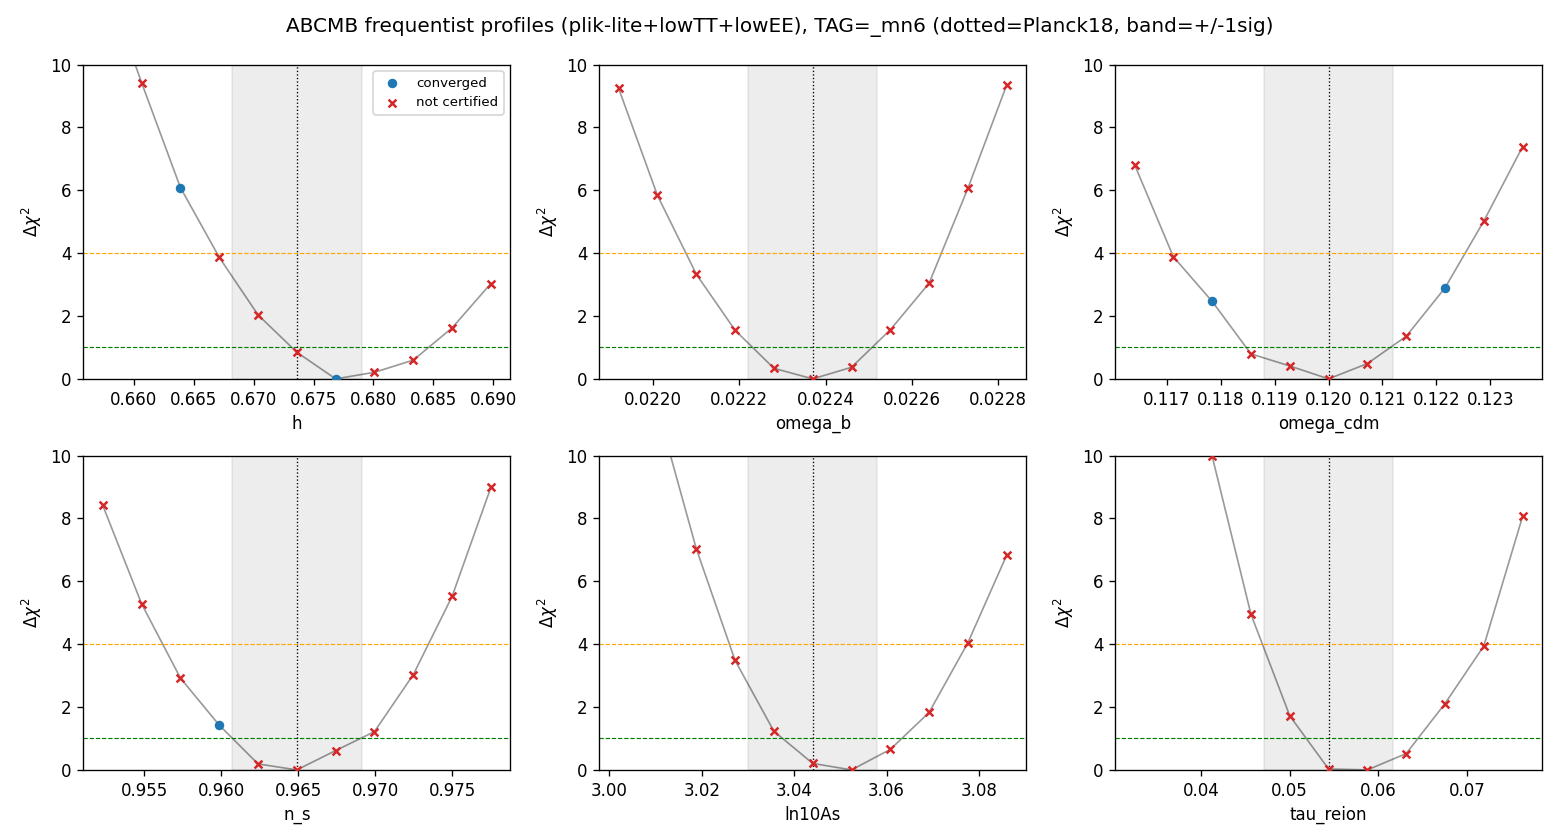
\includegraphics[width=0.95\textwidth]{../results/profiles_summary_mn6.png}
\caption{The six $\Lambda$CDM profile curves $\dchisq(\theta_a)$ with
the $\dchisq=1,4$ levels and the Planck~2018 central value
$\pm1\sigma$ band overlaid (\file{scan/results/profiles\_summary\_mn6.png}).
\emph{This is the profile-likelihood result}: the
$1\sigma$/$2\sigma$ labels assume the Wilks mapping $\dchisq=1,4$
(Section~\ref{sec:wilks}), whose explicit coverage check is the mock study
of Section~\ref{sec:coverage} --- now run, with a first $N{=}500$ pass
confirming these $\Lambda$CDM thresholds.}
\label{fig:headline}
\end{figure}}{%
\par\noindent\textit{[Figure \file{profiles\_summary\_mn6.png} not found at
compile time; it is in \file{scan/results/}.]}\par}

\subsection{Full-\code{plik} cross-check and $\Lambda\mathrm{CDM}+\Neff$}

The same six POIs re-run against the \emph{full} Planck \code{plik}
(clipy, $21$ profiled foreground/calibration nuisances via the SPG
profiler, Section~\ref{sec:spg}) completed cleanly in
$4\,\mathrm{h}\,21\,\mathrm{m}$ on four nodes and reproduces the
\code{plik\_lite} headline --- validating that the envelope-theorem
inner-profile path is consistent with the analytically marginalised
\code{plik\_lite} path. The $\Lambda\mathrm{CDM}+\Neff$ extension exposed
the static-grid degeneracy failure (Section~\ref{sec:mle}): the
full-\code{plik} $\Neff$ run timed out at $10$~h on four nodes, and its
$\Neff$ profile was salvaged from the iteration-15 checkpoint, giving
$\Neff=2.804$ with $1\sigma=[2.705,3.002]$ (the joint optimum sits near
$h\approx0.666$, $\omega_c\approx0.1165$, $\Neff\approx2.83$). The
definitive intervals come from the re-run through the joint-MLE pre-pass,
which was launched to produce clean $1\sigma$ and $2\sigma$ bounds.

\subsection{The Bayesian anchor (SMC)}

The validated \code{plik\_lite} SMC posterior ($6$-dimensional,
$A_{\mathrm{planck}}$ profiled, $\log Z\approx-509.92$) agrees with the
frequentist profile at the $|0.33\sigma|$ level across all six parameters
(the ``vs.\ SMC'' column of Table~\ref{tab:headline}), confirming that
profiling and marginalising give consistent answers for $\Lambda$CDM.

The two full-\code{plik} fast/slow SMC runs ($N=512$) have since completed,
marginalising all $21$ foreground/calibration nuisances at roughly the
\textsc{ABCMB} cost of the lite run --- the nuisance moves reuse the cached
$C_\ell$ (Section~\ref{sec:fastslow}) --- the $27$-dimensional $\Lambda$CDM run
in $5\,\mathrm{h}\,37\,\mathrm{m}$ and the $28$-dimensional $+\Neff$ run in
$6\,\mathrm{h}\,49\,\mathrm{m}$, each on a single four-GPU node. Both reached
$\beta=1$ with a healthy effective sample size (ESS $=437$ and $511$ of $512$)
and left no particles stranded at the out-of-box $\chisq$ wall. Their cosmology
marginals (Table~\ref{tab:smc}) reproduce Planck~2018: every shared parameter of
the $\Lambda$CDM full-\code{plik} run lies within
$\sim0.5\,\sigma_{\mathrm{Planck}}$, and that run independently reproduces the
lite SMC means --- the marginalised analogue of the profile cross-check of
Section~\ref{sec:validation}.

\begin{table}[h]
\centering
\caption{Full posterior marginals (mean$\,\pm\,$std) from the three SMC runs:
plik-lite ($A_{\mathrm{planck}}$ profiled) and the two full-\code{plik} runs
that marginalise all $21$ nuisances. $\mathcal A_s\equiv\ln(10^{10}A_s)$. The
final rows are run-level diagnostics (wall on one four-GPU node). Generated by
\file{scan/analyze\_smc.ipynb}.}
\label{tab:smc}
\begin{tabular}{lrrr}
\toprule
 & plik-lite & full \code{plik} & full \code{plik}\,$+\Neff$\\
\midrule
$h$            & $0.6789\pm0.0062$     & $0.6760\pm0.0053$     & $0.6823\pm0.0108$\\
$\omega_b$     & $0.022385\pm0.000155$ & $0.022357\pm0.000116$ & $0.022427\pm0.000161$\\
$\omega_c$     & $0.11992\pm0.00137$   & $0.12064\pm0.00122$   & $0.11910\pm0.00241$\\
$n_s$          & $0.96479\pm0.00446$   & $0.96365\pm0.00335$   & $0.96487\pm0.00544$\\
$\mathcal A_s$ & $3.0511\pm0.0126$     & $3.0495\pm0.0085$     & $3.0564\pm0.0123$\\
$\tau$         & $0.05887\pm0.00597$   & $0.05666\pm0.00405$   & $0.06315\pm0.00541$\\
$\Neff$        & ---                   & ---                   & $3.045\pm0.142$\\
\midrule
$\log Z$       & $-509.92$   & $-1432.13$  & $-1434.92$\\
ESS\,/\,$N$    & $308/512$   & $437/512$   & $512/512$\\
wall           & $6\,\mathrm{h}\,25\,\mathrm{m}$ & $5\,\mathrm{h}\,37\,\mathrm{m}$ & $6\,\mathrm{h}\,49\,\mathrm{m}$\\
\bottomrule
\end{tabular}
\end{table}

The $+\Neff$ run delivers the headline profile-vs-marginal comparison for the
extension. The nuisance-marginalised posterior gives $\Neff=3.045\pm0.142$ ---
fully consistent with the Standard-Model $3.044$ --- whereas the frequentist
profile minimum sits lower, at $\Neff=2.804$ with $1\sigma=[2.705,3.002]$. The
two are not in tension once the geometry is read correctly: the
$\Neff$--$h$--$\omega_c$ degeneracy is a \emph{skewed} ridge, so the marginal
mean (which integrates the banana) and the profile optimum (which follows its
floor) separate. The same skew moves $h$ --- the SMC marginal
$h=0.682\pm0.011$ sits above the profile MLE $h\approx0.660$, with the profile
optimum the closer match to Planck's own $+\Neff$ marginals. This is the
expected Bayesian-vs-frequentist divergence under a strong degeneracy, not a
defect of either route; it is precisely the comparison the two tools exist to
make, and the triangle plot that exhibits the banana is in
\file{scan/analyze\_smc.ipynb}.

The evidence mildly prefers the base model:
$\Delta\log Z(\Lambda\mathrm{CDM}-{+}\Neff)=+2.79$ on the full \code{plik}
(a Bayes factor $\approx16$, ``positive'' on the Jeffreys scale), consistent
with $\Neff$ being within $1\sigma$ of $3.044$. This number is
\emph{indicative only}: the $+\Neff$ cosmology prior box was recentred and
widened on the joint MLE (Section~\ref{sec:mle}), so its prior volume --- and
hence the Occam factor --- differs from the $\Lambda$CDM run; a clean model
comparison would re-run both under an identical box. The plik-lite
$\log Z=-509.92$ lives in a different parameter and likelihood space and is
\emph{not} comparable to the full-\code{plik} values.

\subsection{Validation summary}
\label{sec:validation}

For a referee-facing read, the correctness story rolls up to five
empirical checks, each documented next to the component it validates (the
convergence guarantees, the Wilks discussion, and the full error budget are
in Section~\ref{sec:rigor}):
\begin{enumerate}[leftmargin=2em,itemsep=1pt]
\item \textbf{Staged AD gradient} vs.\ a single-path \code{jacfwd} of the
same objective: worst relative error $8.58\times10^{-4}$; sharded vs.\
unsharded $\chisq$ to $1.5\times10^{-9}$, gradient to $3.3\times10^{-5}$
(Section~\ref{sec:gradcost}).
\item \textbf{SPG foreground profiler} vs.\ \code{scipy} L-BFGS-B: worst
$\chisq$ gap $0.017$, under the solver roughness floor
(Section~\ref{sec:spg}).
\item \textbf{Full \code{plik}} 6-POI profile reproduces the
analytically-marginalised \code{plik\_lite} headline
(Section~\ref{sec:results}).
\item \textbf{Profile vs.\ SMC}: the frequentist optimum agrees with the
Bayesian posterior mode to $|0.33\sigma|$ across all six $\Lambda$CDM
parameters (Table~\ref{tab:headline}).
\item \textbf{Coverage / Wilks mocks}: the batched coverage validator
(Section~\ref{sec:coverage}) returns a per-mock median test statistic on the
$\chisq_1$ median for the parameters checked --- on GPU at small $N$
($0.530$/$0.358$ vs $0.455$) and in a first $N{=}500$ pass ($0.42$--$0.55$
across $\Lambda$CDM) --- directly corroborating the $\dchisq$ interval
coverage; the full $68\%/95\%$ table is in production.
\end{enumerate}

\subsection{Performance summary}
The throughput numbers (Section~\ref{sec:gradcost}, Table~\ref{tab:throughput})
make a full $\Lambda$CDM six-POI profile a few node-hours (measured:
$2\,\mathrm{h}\,58\,\mathrm{m}$ on six nodes, plik-lite; $4\,\mathrm{h}\,21\,\mathrm{m}$
on four nodes, full plik). A seven-POI $\Lambda\mathrm{CDM}+\Neff$ profile
is \emph{projected} (from the measured 6-POI runs and the cost model) to
land well under the $22$~h CLASS+MH bar on four nodes --- the
definitive Neff timing awaits the joint-MLE-pre-pass re-run --- and it
carries a per-point AD stationarity certificate MH does not provide.

% =====================================================================
\section{The \textsc{ABCMB} interface and worked examples}
\label{sec:interface}

\subsection{Did the interface change with the refactor? (Mostly no.)}
The per-$k$ refactor is \emph{additive} at the API level. The
single-cosmology interface is \textbf{unchanged} from public
\textsc{ABCMB}: you build a \code{Model} with the same keyword options and
call it on a \code{params} dict, getting back the same \code{Output} bundle
(\code{ClTT, ClTE, ClEE, Pk, l, k, BG, PT, params}). The refactor
\emph{adds} \code{Model.call\_batched(params\_list, shard=None,
k\_chunk\_size=100)}, which returns a \code{BatchedOutput} --- the same
spectra with a leading batch axis, but \emph{without} \code{BG}/\code{PT}
(slice \code{params} and rebuild a single \code{Model} call if you need the
per-cosmology background or perturbation table). The only internal breaking
change is that \code{Background.kappa\_func} (a \code{diffrax.Solution}) was
replaced by the tabulated \code{expmkappa\_tab}, read via
\code{Background.expmkappa(lna)} (Section~\ref{sec:keystone}); this affects
only code that reached into the optical-depth solution object directly ---
ordinary $\Cl$/$P_m(k)$ users see no change. Existing single-cosmology
scripts run verbatim.

\subsection{Single cosmology (identical to public \textsc{ABCMB})}
\begin{lstlisting}
import jax; jax.config.update("jax_enable_x64", True)
from abcmb.main import Model

params = {
    "h": 0.6736, "omega_b": 0.02237, "omega_cdm": 0.1200,
    "n_s": 0.9649, "A_s": 2.1e-9, "tau_reion": 0.0544,
    "Neff": 3.044, "YHe": 0.2454, "TCMB0": 2.34865418e-4,
    "N_nu_massive": 1, "T_nu_massive": 0.71611, "m_nu_massive": 0.06,
    "Delta_z_reion": 0.5, "z_reion_He": 3.5,
    "Delta_z_reion_He": 0.5, "exp_reion": 1.5,
}
model = Model(output_Cl=True, l_max=2508, lensing=True,
              output_Pk=True, output_k_max=0.5,
              l_max_g=12, l_max_pol_g=10, l_max_ur=17, l_max_ncdm=17)
out = model(params)                       # -> Output (eqx.Module)
print(out.ClTT.shape, out.l.shape, out.Pk.shape)   # (n_l,), (n_l,), (n_k,)
\end{lstlisting}
Notes: \code{A\_s} is the linear amplitude (the tools sample
$\mathcal A_s=\ln(10^{10}A_s)$ and convert); massive neutrinos are enabled
by \code{N\_nu\_massive>0} (which adds a \code{MassiveNeutrino} species ---
pass it to \code{Model} via the \code{user\_species} tuple for a massive
run); and \code{model.add\_derived\_parameters(params)} returns the dict
with all derived keys filled, if you want to inspect them.

\subsection{Many cosmologies at once (the new batched call)}
\begin{lstlisting}
# vary h across a grid, hold everything else fixed
grid = [dict(params, h=hv) for hv in (0.66, 0.67, 0.68, 0.69)]
bout = model.call_batched(grid)           # shard=None -> auto (multi-GPU if visible)
print(bout.ClTT.shape)                     # (4, n_l)
# bout has ClTT/ClTE/ClEE/Pk/l/k/params; NOT BG/PT
\end{lstlisting}

\subsection{Multi-GPU sharding}
\begin{lstlisting}
# on a 4-GPU node, force B-axis sharding across all visible GPUs:
bout = model.call_batched(big_grid, shard=True)  # B padded to a multiple of n_dev
# shard=None already auto-shards when >1 GPU is visible; shard=False stays single-device
\end{lstlisting}
Always run \textsc{ABCMB} Python on a GPU \emph{compute node} inside an
allocation (never the login node), exporting \code{PYTHONPATH=\$(pwd)} so the
local checkout is imported rather than a sibling install:
\begin{lstlisting}
srun --jobid=$JOBID --ntasks=1 --gpus-per-task=1 bash -c \
  'module load conda && conda activate actdr6 && PYTHONPATH=$(pwd) python myscan.py'
\end{lstlisting}

\subsection{Running the scans (minimal)}
The profile and SMC drivers wrap \code{call\_batched}; you pick the physics
with a config and launch one \code{sbatch}. The minimal forms (full command
set in Section~\ref{sec:usage}):
\begin{lstlisting}
# frequentist profile, 6-POI LCDM, one POI per node (6 nodes):
PA_CONFIG=scan/configs/lcdm.py PA_POI_SLICE=1 PA_NPTS=25 PA_TAG=_run1 \
  sbatch --nodes=6 --ntasks-per-node=1 scan/profile_prod_ad.slurm
python scan/collect_profiles.py _run1     # -> summary table + overlay plot

# Bayesian SMC posterior + evidence (single 4-GPU node):
sbatch scan/smc_lcdm.slurm
\end{lstlisting}

% =====================================================================
\section{Usage cookbook}
\label{sec:usage}

All commands assume the checkout root and an active allocation; prefix
every \code{python} with \code{module load conda \&\& conda activate
actdr6} and export \code{PYTHONPATH=\$(pwd)}. The full env-var references
are Appendices~\ref{app:profenv} (profile) and \ref{app:smcenv} (SMC);
the file map is Appendix~\ref{app:files}.

\paragraph{A $\Lambda$CDM profile (single node)}
\begin{lstlisting}
PA_CONFIG=scan/configs/lcdm.py PA_NPTS=25 \
  python scan/profile_prod_ad.py
\end{lstlisting}

\paragraph{A six-node, one-POI-per-node profile}
The shipped \file{scan/profile\_prod\_ad.slurm} defaults to \code{--nodes=1};
override the node/task count to the number of POIs:
\begin{lstlisting}
PA_CONFIG=scan/configs/lcdm.py PA_POI_SLICE=1 PA_NPTS=11 PA_TAG=_mn6 \
  sbatch --nodes=6 --ntasks-per-node=1 scan/profile_prod_ad.slurm
python scan/collect_profiles.py _mn6   # -> summary table + overlay plot
\end{lstlisting}

\paragraph{A new-physics extension (robust grids)}
\begin{lstlisting}
PA_CONFIG=scan/configs/lcdm_neff.py PA_MLE_PREPASS=1 PA_TAG=_neff \
  sbatch --nodes=7 --ntasks-per-node=1 scan/profile_prod_ad.slurm
\end{lstlisting}

\paragraph{Full Planck plik}
Use a \code{plik\_full} config (\code{high\_ell="plik\_full"}); everything
else is identical.

\paragraph{An SMC posterior}
\begin{lstlisting}
# plik_lite (6-D):
sbatch scan/smc_lcdm.slurm
# full plik, 21 nuisances marginalised (27-D):
SMC_CONFIG=scan/configs/lcdm_plikfull.py sbatch scan/smc_plikfull.slurm
\end{lstlisting}
Both auto-resume from \file{<out>\_state.npz} on resubmission.

% =====================================================================
\section{Gotchas (hard-won)}
\label{sec:gotchas}

\begin{enumerate}[leftmargin=2em,itemsep=2pt]
\item \textbf{Never} \code{jit}/\code{vmap}/\code{jacfwd} the whole
cross-device pipeline --- it fuses the GPU$\to$CPU(HyRex)$\to$GPU stage
into a $\sim20$-min monolith/hang. Stage every jvp per already-jitted
batched stage (Section~\ref{sec:staged}).
\item \code{\_to\_float} every derived-parameter dict before any jvp;
an integer leaf has no tangent and the partition structures mismatch
(Section~\ref{sec:staged}).
\item \textbf{Shard before the setup}, not after, and pad $B$ to a
multiple of $n_{\mathrm{dev}}$ (Section~\ref{sec:sharding}).
\item \textbf{The consistency rule:} all $\chisq$ values from one path
(\code{call\_batched}); AD/FD supplies only directions/curvature
(Section~\ref{sec:consistency}).
\item Batch-shape churn is compile churn ($\sim5$~min per new
$(B,\Lmax)$); pad and mask, keep $B$ stable across iterations and jobs.
\item Keep $k$-chunk at $100$; smaller is slower with no memory benefit.
\item Production \code{rtol\_large\_k\_PE}$=10^{-5}$; $10^{-4}$ biases the
interval midpoint by $\sim19\%$ of $\sigma$. Do \emph{not} chase the
$\sim0.1$ $\chisq$ roughness floor with a tighter \code{rtol} --- it is a
discretisation effect, \code{rtol}-independent, and it averages out of the
intervals.
\item Low-$\ell$ TT/EE carry a large additive constant (min $\chisq\sim1012$
with low-$\ell$ vs.\ $\sim607$ \code{plik\_lite}-only); it cancels in
$\dchisq$ (Section~\ref{sec:lowl}).
\item The full AD Hessian (forward-over-forward) OOMs at $\Lmax=2508$
($\sim35$~GB/cosmo); curvature comes from the BFGS history and the final
co-profiled Hessian from one central FD of the exact AD gradient.
\item The envelope-theorem \code{stop\_gradient} on the nuisance optimum
is exact, not an approximation --- do not ``fix'' it
(Section~\ref{sec:envelope}).
\item Size $\Bloc$ for 40\,GB nodes unless you know the allocation is
80\,GB; a $B=512$ single \code{call\_batched} OOMs on 40\,GB
(Section~\ref{sec:resources}).
\end{enumerate}

% =====================================================================
\section{Directions for improvement}
\label{sec:improve}

The toolkit has a precision/speed dial; this section lists the levers
ordered by effort, and flags which trade against each other. In short:
\emph{speed} comes from larger batches and more nodes (both cheap);
the \emph{interval} precision is already at the $\sim0.02$--$0.03\sigma$
floor, so the next precision gains are the engine-grid knobs and extending
the now-running coverage study (Section~\ref{sec:coverage}) to the bounded
directions; and driving the per-point \emph{certificate} $\ginf$ to
GTOL is the one place where precision costs speed and memory.

\subsection{Easiest speed wins (low effort, no accuracy cost)}
\begin{enumerate}[leftmargin=2em,itemsep=2pt]
\item \textbf{Ride a larger batch $B$.} Per-cosmology cost falls steeply
with $B$ (Table~\ref{tab:throughput}: $1.30\to0.67$ s/cosmo from
$B=64\to256$ at production shape). Raise \code{PA\_AD\_BCHUNK} /
\code{PA\_FD\_CHUNK} (profile) and \code{SMC\_EVAL\_CHUNK} (SMC) toward the
memory ceiling (Section~\ref{sec:resources}); the only cost is GPU memory.
This is the single biggest free lever.
\item \textbf{Add nodes, not walltime.} The profile tool node-slices its
POI list (\code{PA\_POI\_SLICE}, Section~\ref{sec:poislice}); $n$ nodes are
$\approx n\times$ faster up to the POI count. (SMC does not node-slice ---
Section~\ref{sec:spmd}.)
\item \textbf{Keep the $\sigma_1$ early-stop on} (default;
$\sim2.3$--$2.6\times$, Section~\ref{sec:earlystop}). For a model you trust
to be smooth you can loosen \code{PA\_SIGTOL} above $10^{-2}$ for a further
cut --- at the risk of a slightly under-converged interval, so validate
once.
\item \textbf{Warm-start the inner SPG across outer BFGS iterations}
(full-\code{plik} only). The foreground nuisances barely move between outer
iterations, so seeding SPG from the previous iteration's $\nu^\star$ cuts
its $\sim800$ steps by a large factor. This is the documented next speed
lever for full-\code{plik}; it is not yet wired.
\item \textbf{Precompute the warm/MLE Hessian once and reuse it} across
ranks/runs. It is already disk-cached (loads in $\sim0$~s); precomputing it
for a fresh multi-node run avoids each rank paying the $\sim18$~min build
(Section~\ref{sec:lockstep}).
\item \textbf{Keep batch shapes stable} so the $\sim5$~min staged-jvp
compile is paid once and the persistent compile cache is hit on restart
(Section~\ref{sec:resources}).
\end{enumerate}

\subsection{Easiest precision and rigor wins}
\begin{enumerate}[leftmargin=2em,itemsep=2pt]
\item \textbf{Finish and extend the coverage mocks} (Section~\ref{sec:coverage}).
The validator is built and validated and the $\Lambda$CDM /
$\Lambda\mathrm{CDM}+\Neff$ production runs are in flight; what remains is
collecting the full $68\%/95\%$ tables and extending the study to the
\emph{bounded} directions ($\Neff$, $\sum m_\nu$, $r$, $f_{\mathrm{EDE}}$),
where Wilks is expected to fail and the Feldman--Cousins thresholds it
measures are the actual deliverable.
\item \textbf{Denser grids: raise \code{PA\_NPTS}.} More points (e.g.\
$25$--$31$ vs $11$) reduce the PCHIP spline's interpolation error and better
bracket $\dchisq=1,4$ --- nearly free on the batch axis.
\item \textbf{Use the MLE pre-pass and multistart}
(\code{PA\_MLE\_PREPASS}, \code{PA\_MULTISTART}; Sections~\ref{sec:mle},
\ref{sec:cert}). The pre-pass centres grids on the joint optimum (essential
for new degenerate parameters); multistart upgrades the global-minimum
claim from a check to a certificate.
\item \textbf{Do not loosen \code{PA\_RTOL} below $10^{-5}$} --- and do not
bother tightening it for the roughness floor: the $\sim0.1$ $\chisq$
roughness is \code{rtol}-independent (proven), so $10^{-6}$ buys nothing
there while costing runtime. ($10^{-4}$ is off-limits --- it biases the
midpoint by $\sim19\%$ of $\sigma$.)
\end{enumerate}

\subsection{Tightening the per-point certificate (precision that costs speed)}
The AD $\ginf$ floors at $\sim1$--$5$ rather than reaching
$\mathrm{GTOL}=0.03$ because of the $\sim0.1$ $\chisq$ discretisation
roughness, whose source is the $k$-chunking and the visibility-driven
$\ln a$ grid (\emph{not} the ODE tolerance). This does \emph{not} bias the
interval (it averages out, Section~\ref{sec:errbudget}), so it only matters
if you want the certificate itself to reach GTOL. To reduce it:
\begin{itemize}[leftmargin=1.5em,itemsep=1pt]
\item Increase the save-grid resolution: revert the round-4 engine default
to \code{n\_lna\_PE=500} with \code{lna\_grid\_mode="uniform"} (the current
$300$/visibility default traded a sub-permille $\ell<5$ quadrupole
regression and $\sim1.65\times$ memory for speed). This is also the lever
for better low-$\ell$ precision (EE at $\ell=2$).
\item Densify the perturbation $k$-axis. Both raise per-call memory and
runtime, so they trade directly against the speed levers above; pursue them
only if a GTOL-level certificate is required.
\end{itemize}
The tension is real: the round-3/round-4 work cut per-call memory
$\sim2\times$ then $\sim1.65\times$ precisely to \emph{enable} larger $B$
(speed), partly by \emph{lowering} grid resolution. Pushing the certificate
precision here gives that memory back.

\subsection{Larger refactors (higher effort, on the table)}
\begin{itemize}[leftmargin=1.5em,itemsep=1pt]
\item \textbf{Stream the perturbation table per $k$-chunk} (``Idea~A2'')
instead of holding the full $(B,N_y,N_{\ln a},N_k)$ tensor: it would cut
the binding per-device memory $\propto N_k$, directly enabling larger $B$
(hence speed). It is blocked by the spectrum's global cubic spline over the
$k$-axis, so it needs a chunk-aware spectrum integrator --- a genuine
refactor.
\item \textbf{Hybrid FD/AD gradients for non-stiff models.} Central FD on
the batch axis is $\sim2\times$ cheaper per direction than AD \emph{when it
calibrates below the noise floor} (Section~\ref{sec:advsfd}); for a
well-behaved model at lower $\ell$, \code{grad\_method="fdbatch"} with the
final AD certificate is a speed win. (At $\Lmax=2508$ base $\Lambda$CDM it
does not calibrate, which is why the shipped configs use \code{"ad"}.)
\item \textbf{LINX under \code{vmap}} for large-$B$ \code{bbn\_type="linx"}
scans. LINX currently runs per-cosmology in the eager
\code{add\_derived\_parameters} loop ($\sim$ms each, fine now); a vmapped
BBN stage would matter for big batches that solve BBN per cosmology.
\item \textbf{Intra-POI row-slicing} across nodes for parallelism beyond
the POI count, which needs an MPI gather (Section~\ref{sec:future}).
\end{itemize}

\begin{center}
\begin{tabular}{p{0.28\textwidth}p{0.14\textwidth}p{0.48\textwidth}}
\toprule
goal & effort & lever \\
\midrule
faster & trivial & larger $B$ (chunk knobs); more nodes (POI-slice); keep $\sigma_1$ early-stop \\
faster (full plik) & low & warm-start SPG across outer iters; precompute+broadcast the Hessian \\
faster & high & stream PT per $k$-chunk (Idea~A2); hybrid FD/AD \\
more rigorous & low & coverage mocks; multistart; MLE pre-pass \\
tighter interval & trivial & denser grid (\code{PA\_NPTS}) \\
tighter certificate & medium & \code{n\_lna\_PE=500}+uniform grid; denser $k$-axis (costs memory/speed) \\
\bottomrule
\end{tabular}
\end{center}

% =====================================================================
\section{Planned work}
\label{sec:future}

\paragraph{Coverage mocks (Feldman--Cousins / Wilks validation)}
\emph{Implemented and validated} since the introduction was first drafted
(Section~\ref{sec:coverage}): the batched validator is built, its
shared-Jacobian fitter is GPU-checked, and the $\Lambda$CDM and
$\Lambda\mathrm{CDM}+\Neff$ production runs are in flight. What remains is
collecting the final $68\%/95\%$ coverage tables and extending the
construction to the bounded-parameter directions ($\Neff$, $\sum m_\nu$,
$r$, $f_{\mathrm{EDE}}$), where the measured Feldman--Cousins thresholds ---
not Wilks --- are the deliverable.

\paragraph{Other open items}
LINX under \code{vmap} for large-$B$ \code{bbn\_type="linx"} scans (LINX
currently runs per-cosmology in the eager \code{add\_derived\_parameters}
loop, fine at $\sim$ms/cosmo); and an intra-POI row-slice for $>$6-way
parallelism (needs an MPI gather).

% =====================================================================
\appendix
\section{Profile-tool environment variables}
\label{app:profenv}

The principal \code{PA\_*} knobs read by \file{scan/profile\_prod\_ad.py}
(the script exposes additional debug/legacy variables --- e.g.\
\code{PA\_FD\_CHUNK}, \code{PA\_HESS\_CACHE}, \code{PA\_FTOL}/\code{PA\_FTOL\_PATIENCE},
\code{PA\_MLE\_MAXITER}, \code{PA\_MS\_K}, \code{PA\_HIGH\_ELL},
\code{PA\_RANK\_SLICE}, \code{PA\_WARM\_DIR}, \code{PA\_BF\_TRACE} --- not
listed here):
\begin{longtable}{p{0.26\textwidth}p{0.14\textwidth}p{0.50\textwidth}}
\toprule
env var & default & meaning \\
\midrule
\endhead
\code{PA\_CONFIG} & \code{configs/lcdm.py} & config module \\
\code{PA\_POIS} & config \code{pois} & POIs to profile (csv) \\
\code{PA\_NPTS} & $25$ & grid points per POI \\
\code{PA\_NSIG} & $3.0$ & grid half-extent in $\sigma$ \\
\code{PA\_LMAX} & $2508$ & theory $\Lmax$ \\
\code{PA\_MAXIT} & $40$ & max BFGS iterations \\
\code{PA\_GTOL} & $3\times10^{-2}$ & $\ginf<$GTOL convergence gate \\
\code{PA\_SIGTOL} & $10^{-2}$ & $\sigma_1$-stability early-stop tol ($\sigma$-units) \\
\code{PA\_SIGTOL\_PATIENCE} & $3$ & early-stop window $W_{\mathrm{pat}}$ \\
\code{PA\_RTOL} & $10^{-5}$ & perturbation \code{rtol\_large\_k\_PE} \\
\code{PA\_GRADMETHOD} & (config) & debug override of \code{grad\_method} (warns) \\
\code{PA\_AD\_BCHUNK} & $64$ & batch per staged-AD block \\
\code{PA\_GRAD\_KCHUNK} & $100$ & $k$-chunk for the AD gradient \\
\code{PA\_FD\_STEP} & $10^{-2}$ & central-FD step (scaled) \\
\code{PA\_FD\_CALTOL} & $10^{-2}$ & FD-vs-AD calibration target \\
\code{PA\_PRECOND} & $1$ & inverse-Fisher preconditioner \\
\code{PA\_HESS} & $1$ (code); $0$ in prod slurm & co-profiled Hessian / PD check \\
\code{PA\_WARM} & $1$ & use warm starts \\
\code{PA\_WARM\_FROM\_CEN} & $0$ & warm-start from config centre \\
\code{PA\_MLE\_PREPASS} & $0$ & joint-MLE auto-centering pre-pass \\
\code{PA\_MULTISTART} & $0$ & multistart global-min check \\
\code{PA\_POI\_SLICE} & $0$ & multi-node POI striping \\
\code{PA\_USE\_LOWTT} & config (True) & include low-$\ell$ TT \\
\code{PA\_USE\_LOWEE} & config (True) & include low-$\ell$ EE \\
\code{PA\_TAG} & \texttt{""} & output filename suffix \\
\code{PA\_RESUME} & $1$ & resume from checkpoint \\
\bottomrule
\end{longtable}

\section{SMC environment variables}
\label{app:smcenv}
\begin{longtable}{p{0.26\textwidth}p{0.18\textwidth}p{0.46\textwidth}}
\toprule
env var & default & meaning \\
\midrule
\endhead
\code{SMC\_N} & $512$ & particles (fixed for the run) \\
\code{SMC\_EVAL\_CHUNK} & $128$ & cosmologies per \code{call\_batched} \\
\code{SMC\_CLIPY\_CHUNK} & $32$ & nuisances per batched clipy eval (full plik) \\
\code{SMC\_MOVES} & $3$ & MH moves/stage (\code{smc.py}) \\
\code{SMC\_MOVES\_SLOW} & $2$ & cosmology (theory) moves/stage (full plik) \\
\code{SMC\_MOVES\_FAST} & $20$ & nuisance (clipy-only) moves/stage (full plik) \\
\code{SMC\_ESS\_TARGET} & $0.5$ & ESS target fraction of $N$ \\
\code{SMC\_MAXSTAGES} & $80$/$120$ & max tempering stages (lite/full) \\
\code{SMC\_PRIOR\_NSIG} & $5.0$ & cosmology flat-box half-width ($\sigma$) \\
\code{SMC\_NUIS\_BOX\_NSIG} & $6.0$ & unbounded-nuisance box half-width ($\times$scale) \\
\code{SMC\_TAU\_FLOOR} & $0.01$ & $\tau$ lower-edge floor \\
\code{SMC\_LMAX} & $2508$ & theory $\Lmax$ \\
\code{SMC\_RTOL} & $10^{-5}$ & perturbation tolerance \\
\code{SMC\_SEED} & $0$ & RNG seed \\
\code{SMC\_SHARD} & auto & shard if $>1$ GPU \\
\code{SMC\_CONFIG} & lite/full config & config module \\
\code{SMC\_OUT} & \code{results/smc\_*} & output prefix \\
\bottomrule
\end{longtable}

\section{File map}
\label{app:files}
\begin{longtable}{p{0.36\textwidth}p{0.58\textwidth}}
\toprule
file & role \\
\midrule
\endhead
\file{abcmb/main.py} & \code{Model.call\_batched}, \code{\_make\_shardfn},
\code{\_build\_bgs\_batched}, \code{BatchedOutput}, \code{add\_derived\_parameters} \\
\file{abcmb/perturbations.py} & \code{full\_evolution\_batched},
\code{\_evolve\_chunk} ($k$-chunking) \\
\file{abcmb/spectrum.py} & \code{get\_Cl\_batched}, \code{Pk\_lin\_batched} \\
\file{abcmb/background.py} & \code{expmkappa\_tab} keystone \\
\file{scan/batched\_grad.py} & staged forward-mode gradient
(\code{staged\_cl\_and\_grad}, \code{staged\_chi2\_and\_grad}) \\
\file{scan/profile\_prod\_ad.py} & the profile-likelihood driver \\
\file{scan/profile\_prod\_ad.slurm}, \file{scan/profile\_prod\_plikfull.slurm} & SLURM drivers for the profile tool (lite / full plik) \\
\file{scan/collect\_profiles.py} & per-POI $\to$ summary table + overlay plot \\
\file{scan/smc.py} & plik-lite SMC ($6$-D) \\
\file{scan/smc\_plikfull.py} & full-plik fast/slow Gibbs SMC ($27$/$28$-D) \\
\file{scan/smc\_lcdm.slurm}, \file{scan/smc\_plikfull.slurm} & SLURM drivers for the SMC tools \\
\file{scan/analyze\_smc.ipynb} & SMC posterior analysis notebook (health, marginals
vs Planck/profile, triangle, nuisance pulls, evidence; CPU-only). Regenerate with
\file{scan/make\_analyze\_smc\_nb.py} \\
\file{scan/wilks.py} & coverage / Wilks validator: batched shared-Jacobian
Gauss--Newton, per-mock-J cert (Section~\ref{sec:coverage}) \\
\file{scan/wilks\_collect.py} & pool node slices $\to$ coverage table + plots \\
\file{scan/wilks.slurm} & SLURM driver for the coverage runs \\
\file{scan/wilks\_analysis.ipynb} & coverage analysis notebook (per-POI coverage
tables, $t$ vs $\chisq_1$, pull vs $\mathcal N(0,1)$, the per-mock-J cert; CPU-only) \\
\file{scan/plik\_lite.py} & plik-lite likelihood + analytic $A_{\mathrm{planck}}$ \\
\file{scan/plik\_full.py} & full plik (clipy) + SPG nuisance profiler \\
\file{scan/lowl\_like.py} & low-$\ell$ TT (Commander) + EE (SRoll2) \\
\file{scan/configs/*.py} & run configurations \\
\bottomrule
\end{longtable}

% =====================================================================
\begin{thebibliography}{9}

\bibitem{Herold2022} L.~Herold, E.~G.~M.~Ferreira \& E.~Komatsu,
``New Constraint on Early Dark Energy from Planck and BOSS Data Using the
Profile Likelihood,'' \emph{ApJL} \textbf{929}, L16 (2022),
arXiv:2112.12140.

\bibitem{GomezValent2022} A.~G\'omez-Valent,
``A fast test to assess the impact of marginalization in Monte Carlo
analyses, and its application to cosmology,'' \emph{Phys.\ Rev.\ D}
\textbf{106}, 063506 (2022), arXiv:2203.16285.

\bibitem{Nygaard2023} A.~Nygaard, E.~B.~Holm, S.~Hannestad \& T.~Tram,
``Fast and effortless computation of profile likelihoods using the random
walk Metropolis algorithm'' (2023), arXiv:2308.06379.

\bibitem{Holm2024} E.~B.~Holm, A.~Nygaard \emph{et al.},
``PROSPECT: A profile likelihood code for frequentist cosmological
parameter inference,'' \emph{MNRAS} \textbf{535}, 3686 (2024),
arXiv:2312.02972.

\bibitem{Karwal2024} T.~Karwal \emph{et al.},
``Procoli: Profiles of cosmological likelihoods'' (2024),
arXiv:2401.14225.

\bibitem{DMb2026} ``CMB constraints on dark matter--proton scattering:
investigating prior-volume effects using profile likelihoods'' (2026),
arXiv:2603.25731.

\end{thebibliography}

\end{document}
